% This is samplepaper.tex, a sample chapter demonstrating the
% LLNCS macro package for Springer Computer Science proceedings;
% Version 2.21 of 2022/01/12
%
\documentclass[runningheads]{llncs}
%
\usepackage[T1]{fontenc}
% T1 fonts will be used to generate the final print and online PDFs,
% so please use T1 fonts in your manuscript whenever possible.
% Other font encondings may result in incorrect characters.
%
\usepackage{graphicx}
\usepackage{hyperref}
\usepackage{subfig}
\usepackage{booktabs}
\usepackage{amsmath}
\usepackage{bm}
\usepackage{dsfont}
\usepackage{algorithm}
\usepackage{algorithmic}
\usepackage{todonotes}
\usepackage{svg}

% Revision markup: changed or new text is red (xcolor is loaded by todonotes).
\newcommand{\rev}[1]{\textcolor{red}{#1}}

%
\begin{document}
%

\title{Energy-Efficient Flocking in Self-Organized Robot Swarms}
%

\titlerunning{Emergent Energy-Efficient Flocking}
% If the paper title is too long for the running head, you can set
% an abbreviated paper title here
%
\author{
Lilly Schwarzenbach\inst{1} \and
Sina Mahdavi\inst{2} \and
%Dushyant Singh\inst{1} \and
%Peter Klapwijk\inst{1} \and
Georges Jetti\inst{2}\orcidID{0009-0007-9682-4838} \and
Michael Khayyat\inst{2}\orcidID{0000-0002-1718-4198} \and
Francesco Braghin\inst{2}\orcidID{0000-0002-0476-4118} \and
Eliseo Ferrante\inst{1,3}\orcidID{0000-0002-2213-8356}}

%
\authorrunning{L.Schwarzenbach et al.}
% First names are abbreviated in the running head.
% If there are more than two authors, 'et al.' is used.
%
\institute{ Vrije Universiteit Amsterdam, Amsterdam, The Netherlands\\
\email{l.m.schwarzenbach@vu.nl}\and
Politecnico di Milano, Milan, Italy \and
New York University Abu Dhabi, Abu Dhabi, United Arab Emirates
}

\index{Schwarzenbach, Lilly}
\index{Mahdavi, Sina}
%\index{Singh, Dushyant}
%\index{Klapwijk, Peter}
\index{Jetti, Georges}
\index{Khayyat, Michael}
\index{Braghin, Francesco}
\index{Ferrante, Eliseo}
%
\maketitle              % typeset the header of the contribution
%
\begin{abstract} % 150-250 words

Groups of natural agents such as flocks of birds preserve energy by changing positions and thereby taking turns being exposed to the wind. We evolve an energy-aware controller for decentralized, memoryless, communication-free agents in a 2D environment. Our results show that being aware of neighbours' range and bearing, a digital compass and the battery level is enough to produce emergent reconfigurations akin to those observed in natural groups\rev{: in a swarm of 20 robots, the robot at the exposed front changes about ten times per minute, almost five times as often as in a traditional flocking baseline model}.
We validate our model in simulation and real Thymio-II robots. \rev{In simulation with 20 robots, the evolved controller travels more than twice as far as the baseline before the first robot runs out of battery, while also retaining more battery. This advantage depends on swarm size: it appears only from about 13 robots upwards, and in small swarms the baseline performs better. For the real robots, we evolve a second controller under a speed clamp that prevents collisions; it still travels $59\%$ further than the baseline in simulation.}

\end{abstract}
%
%
%
\section{Introduction}
One of the fundamental behaviours in robot swarms is that of collective motion, allowing a group of robots to move in an aligned fashion as a group\cite{vicsek-col-motion}. This offers numerous benefits, such as enhanced foraging \cite{couzin2005effective}, predator evasion \cite{olson2013predator}, efficient navigation \cite{couzin2005effective}, and improved hydrodynamic and aerodynamic performance \cite{beaver2021overview}.

However, animals and robots share a central limitation: Their movement is limited by the amount of energy at their disposal. Moving costs energy. Animals need to rest and feed to recharge; robots need to charge at a charging station or have their batteries changed. However, these activities cost time and in the case of robots, may require human intervention which is inconvenient especially in environments that are less accessible to humans such as cave systems, aerial or underwater inspection systems. It is therefore paramount to save energy wherever possible. For this purpose, we take inspiration from animals that have already developed energy-efficient behaviours such as bird flocks, fish schools, and insect colonies. They have a few things in common: They are fully decentralised, interactions are purely local, there are no explicit leaders, and there is no explicit communication. These assumptions are in line with those made by swarm robotics, which is known to produce scalable and cost-effective solutions\cite{Brambilla2013,Dorigo2021,Debie2023,FariaDias2021}. Therefore, it is only natural that researchers look to natural collective systems for understanding and design inspiration for swarm robotics applications\cite{Andersson2004,Voelkl2017,Mirzaeinia2020,Hassanalian2022,Beaumont2024,Friman2024}.

Previous work has identified dynamic reconfiguration as one of the key factors contributing to the improved aerodynamic performance in collective navigation\cite{beaver2021overview}. If the agents stay in the same positions throughout their journey, environmental effects remain unevenly distributed. In the case of migratory birds, the front positions are more energy-draining. By periodically changing positions, this energy drain can be distributed among agents and the individual agents lose less energy. Using this strategy, migratory birds save about 11-71\% energy depending on their position within the flock, while the flock itself can extend its flight range by up to 44.6\%~\cite{Voelkl2017,Mirzaeinia2020,Beaumont2024,Zhang2024}. Similar mechanisms appear in human cycling pelotons~\cite{Blocken2018}.

Although there is evidence for the importance this reconfiguration behaviour, the literature in swarm robotics has considered energy efficiency and formation reconfiguration in isolation and not together with the exception of~\cite{mahdavi2026energy}, which we extend and further validate here.

Energy efficiency has been addressed in multiple ways in swarm robotics. Among other approaches, energy has been proposed as a proxy for a reward rather than a physical property which would cause the robots to fail~\cite{Elfwing2005,Weel2012,Haasdijk2013}. Another approach shows that using energy levels allows response-threshold policies to improve efficiency in self-assignment to either foraging or resting~\cite{Wenguo2007}. Other studies have proposed to tackle energy efficiency by optimising the hardware and the use of perception and communication~\cite{Yasin2021,Zhang2023,Ren2024}.

Formation reconfiguration is an active field in multi-robot systems but has not been widely explored under the more stringent requirements of swarm robotics. The v-shape common in flocks of birds specifically has been targeted in multiple works.
Yang et al. (2016)\cite{Yang2016} use MPC and achieve V-formation by optimizing over velocity matching between agents, clear view, and upwash benefit, in both centralized and decentralized frameworks. Roy et al. (2020)\cite{Roy2020} optimize a similar cost function and propose a learning based framework that combines MPC with DNC as a teacher-learner pair. Although these works were able to achieve the V-shaped flocking pattern using simple local rules, dynamic formation reconfiguration is missing from them. In addition, they required full knowledge of the aerodynamic landscape. Instead, a greedy leading/trailing replacement heuristic was proposed by Mirzaeinia et al. (2019)\cite{Mirzaeinia2019} to achieve dynamic formation reconfiguration using battery thresholds. Then, Liu et. al. (2024)\cite{Liu2024}\cite{2Liu2024} frame the same issue as an optimization problem but require the energetic cost of the positions as input. However, both works assumed particular fixed patterns, such as the V-formation, and solved dynamic position assignment within the confines of these formations. Also, they took advantage of global communication between members.

In this work, we address the problem of energy-efficient collective motion by evolving a controller for simple, memory-less robots in a 2D environment with uniform wind. The wind as well as the motion drains the battery and the group can only move while all of the robots still have battery.
We use an existing evolutionary swarm robotics framework first proposed in~\cite{vandiggelen2025emergentheterogeneousswarmcontrol}. Our contribution lies in applying this framework to a novel problem: Using only range and bearing sensors and a battery monitoring sensor, travel as far as possible as a group. The robots cannot sense the wind that contributes to the battery being drained nor do they have any information about the state of the other robots. \rev{Extending~\cite{mahdavi2026energy}, we evolve the controller with a two-stage curriculum that rewards moving against the wind from the start, and we evolve a second version under a speed clamp so that it can run safely on real robots.} We show that this is enough for dynamic reconfiguration to emerge and this strategy allows the group to travel further than a traditional flocking baseline model\rev{, and we quantify the reconfiguration with leadership metrics from studies of bird flocks. We also show that the advantage depends on the size of the swarm: controllers evolved with 20 robots outperform the baseline only in large swarms.}


This paper is organised as follows: Section~\ref{sec:methodology} presents the methodology and metrics, Section~\ref{sec:EXp_Setup} introduces the simulation environment and the setup for the real robot experiments as well as the model of the battery drainage. Subsequently, Section~\ref{sec:Exp:Results} presents our findings and finally, Section~\ref{sec:Conclusion} summarises our findings and draws conclusions from them.


\section{Methodology}
\label{sec:methodology}
The methodology is heavily based on the framework presented in~\cite{vandiggelen2025emergentheterogeneousswarmcontrol}, whereby robots are equipped with neural controllers whose weights are updated by Hebbian learning rules, and a separate outer‑loop evolutionary optimizer is used to learn the Hebbian learning update rules. All evolutionary and simulated validation experiments are performed in a 2D kinematic Python simulator\rev{, a port of the MATLAB code of~\cite{mahdavi2026energy}}.
The full workflow is depicted in Fig.~\ref{fig:ES_overview}.

% CHECK: if ES_layout.png still shows the old three-stage pipeline, replace it with
% figures/method_pipeline (upload figures/method_pipeline.pdf from the repo).
\begin{figure}[t]
\centering
\includegraphics[width=1\textwidth]{Images/Methodology/ES_layout.png}
\caption{\textbf{Overview of the Methodology.}
    Our setup comprises a swarm with robots, each equipped with a neural network controller. Each swarm shares one set of Hebbian learning rules, which are learned by the CMA-ES algorithm through evolution. The robots are simulated in the windy arena for fitness calculation.} \label{fig:ES_overview}
\end{figure}

\subsection{Individual Robot Neural Controller}
We consider differential-drive ground robots, whose locomotion capabilities are regulated by forward velocity $v^i$ and angular velocity $\omega^i$.

\begin{figure}[t]
  \centering
  \subfloat[Bearing\label{fig:bearing}]{
    \begin{minipage}[t]{0.35\textwidth}
       \centering
      \includegraphics[width=0.7\linewidth]{Images/Methodology/quadrants.png}
    \end{minipage}
  }
  \subfloat[Range\label{fig:range}]{
    \begin{minipage}[t]{0.35\textwidth}
      \centering
      \includegraphics[width=0.7\linewidth]{Images/Methodology/quadrants_range.png}
    \end{minipage}
  }
  \caption{Sensing capabilities of the individual robots.}
  \label{fig:quadrants}
\end{figure}

The perception capabilities of the robots are as follows: Every robot can perceive neighbours only when they are within a sensing radius $R$ (in our experiments $R=2.01$\rev{\,m)}. $R$ defines a sensing circle that is divided into 4 equal quadrants $q \in [1,2,3,4]$\rev{, centred on the robot's front, left, back and right}. In each quadrant, a sensor gives the distance, $d_q \in [0, R]$, and bearing, $\psi_q \in [0, \pi/2]$, of the nearest neighbour in that quadrant (see Fig.~\ref{fig:quadrants}). \rev{All other neighbours are ignored.} The robot is battery-aware, that is, it senses its remaining battery percentage, $B_0 \in [0, 100]$. The last sensor that is added to the robot
is a digital compass, $\theta_0 \in (-\pi, \pi]$ that provides an approximate task direction context. \rev{Sensing is noise-free in simulation; on the real robots the same inputs are computed from motion-capture poses (Section~\ref{sec:EXp_Setup}).}

Each robot runs a 10-10-10-2 Multi-Layer Perceptron (MLP) with ReLU hidden layers and tanh outputs. The $10$-dimensional inputs to the neural network for agent $i$ will be the 8 local sensory readings of all 4 quadrants ($d^i_q, \psi^i_q$), the battery of the agent ($B^i_0$), and the heading of the agent ($\theta^i_0$). The default input (sensory reading) for when there is no neighbour in a quadrant is $d^i_q=R$, and $\psi^i_q=0$. The ten inputs are rescaled to $[-1,1]$ \rev{($2d/R-1$, $4\psi/\pi-1$, $B/50-1$ and $\theta/\pi$)}. The input layer is followed by two hidden layers with 10 neurons each. The output layer contains two neurons: the first outputs the linear velocity $v^i$ and the second one the angular velocity $\omega^i$ of the agent, which are then rescaled to $v^i \in[-0.2,0.2]$ m/s and $\omega^i \in[-\pi/5,\pi/5]$ rad/s. The MLP has $220$ weights \rev{and no biases. The weights are} randomly initialized at the beginning of each \rev{simulation, independently for every robot,} using a uniform distribution in $[-1,1]$. Each NN weight of every robot is updated \rev{at every time step} using a Hebbian learning update rule. As~\cite{vandiggelen2025emergentheterogeneousswarmcontrol}, we use the Hebbian learning update in Eq.~\ref{eq:hebbian}, where $\delta w_{i,j}$, is the weight change corresponding to the connection between pre- and post-synaptic neurons $i$ and $j$, $\mu$ is the constant learning rate, $n_i$ and $n_j$ are the activations of the neurons, and $A_{i,j},B_{i,j},C_{i,j},D_{i,j}$ are the 4 Hebbian learning update rules or genotype which from now on we shall refer to as ABCD-rules for simplicity.
Each robot will have a different set of NN weights that will vary under the effect of ABCD-rules during its own experience. We keep normalising the weights to prevent unbounded growth during the simulation \cite{leung2025bioinspiredplasticneuralnetworks}\rev{: after each update, any layer whose largest absolute weight exceeds 1 is divided by that value}.
\begin{equation}
    \delta w_{i,j}=\mu(A_{i,j}n_in_j+B_{i,j}n_i+C_{i,j}n_j+D_{i,j})
    \label{eq:hebbian}
\end{equation}

The ABCD-rules vary across each weight of the NN, resulting in 880 parameters (4 for each of the 220 weights) that need to be optimized for the entire swarm.
In particular, the swarm shares the genotype of these 880 parameters, which allows the evolutionary algorithm to scale independently from the swarm size \cite{vandiggelen2025emergentheterogeneousswarmcontrol}.


\subsection{The Evolutionary Algorithms}
The Hebbian learning update parameters are optimized using Covariance Matrix Adaptation Evolution Strategy (CMA-ES) \cite{Hansen2001}. Each generation evaluates a population size $\lambda$ of 30 candidate solutions, where each candidate solution represents a complete set of 880 ABCD parameters that define the Hebbian learning rules for all agents in a swarm. At the beginning of the evolutionary process, the ABCD-rules are sampled uniformly from $[-5, 5]$\rev{, and they are kept within these bounds throughout evolution}. The fitness $f$ of each candidate is evaluated by running 3 simulations (each with a different random seed) of a swarm of 20 agents at full battery until one agent's battery depletes to zero. The fitness $f$ of each candidate is determined as the median of the 3 runs, while the individual fitness of each simulation is calculated as explained in Section \ref{sec:stages}.

\rev{CMA-ES then ranks the candidates and uses the best $\lambda/2 = 15$, combined with rank-based weights, to update its search distribution, from which it samples 30 new ABCD-rules for the next generation. This selection is not elitist: parents are not carried over into the next generation. The best candidate ever evaluated is recorded separately and becomes the result of the stage, rather than the best of the last generation.}
A summary of other Evolution parameters can be found in Table~\ref{tab:swarm_experiment}.

\begin{table}[t]
    \centering
    \caption{Evolving swarm experiment parameters for every stage.}
    \begin{tabular}{llc}
    \toprule
         \textbf{Parameter} & \textbf{Description} & \textbf{Value}\\
        \midrule
        $N_{ABCD}$ &   Number of rules & $880$\\
        $\lambda$  & Population size &  $30$\\
        $N_{\text{gen}}$  & Termination condition & \rev{$100$ (stage 1), $200$ (stage 2)}\\
        $\sigma_0$  & Initial covariance value & $0.3$\\
        $N_{\text{repeats}}$  & Number of repeats per individual & $3$\\
        $\mu$  & Hebbian learning rate & $0.1$\\
        \rev{$N$}  & \rev{Swarm size during evolution} & \rev{$20$}\\
        \bottomrule
    \end{tabular}
    \label{tab:swarm_experiment}
\end{table}


\begin{table}[t]
\centering
\caption{Fitness function during each evolution stage}
\begin{tabular}{cll}
\toprule
\textbf{Stage} & \textbf{Goal} & \textbf{Fitness function}  \\
\midrule
{\color{red}1} & {\color{red}Walk upwind (wind on)} &
{\color{red}$ f = 16\, x_{\text{avg}} $}  \\
{\color{red}2} & {\color{red}\begin{tabular}[c]{@{}l@{}} Save battery and avoid all collision \end{tabular}} &
{\color{red}$ f = 16\, x_\text{{avg}} + \dfrac{B_\text{{avg,end}}}{5} - \dfrac{t_\text{{col}} + 3  \cdot t_\text{{wcol}}}{250} $}  \\
\bottomrule
\end{tabular}
\label{tab:fitness_evolution}
\end{table}


\subsection{Evolutionary Stages}
\label{sec:stages}

In this paper, we perform staged evolutionary experiments, meaning that we consider \rev{two} stages whereby the complexity of the task increases from one stage to the next. This corresponds to a different fitness function in each stage. \rev{Stage 2 starts from the best ABCD-rules found in stage 1.} At the end of each simulation during evolution, the following set of data is recorded that is used to formulate the fitness function: collision time $t_{\text{col}}$, border collision time $t_{\text{wcol}}$, distance travelled towards the left $x_{\text{avg}}$ and remaining battery $B_{\text{avg,end}}$, both averaged over all the agents. \rev{Here $x_{\text{avg}}$ is the distance that the swarm's centroid has moved to the left of the origin, i.e.\ against the wind. Two robots are in collision whenever their centres are less than $0.12$\,m apart, and $t_{\text{col}}$ adds $\Delta t$ for every colliding pair in every time step. $t_{\text{wcol}}$ does the same for every robot touching a wall. In both stages the distance is weighted by 16, so that progress dominates battery saving: robots that stand still drain their battery only at the idle rate, so without this weight the fitness would reward staying put.}

\rev{In stage 1, the wind model is already active, and the fitness rewards only moving towards a target that is assumed to be on the left, i.e.\ directly against the wind, recalling that the robots have no sensor to detect the wind. Because the reward is progress against the wind, the trivial strategy of moving with the wind scores negatively from the start. In stage 2, the fitness combines distance, average remaining battery, and penalties on both wall collisions and inter-robot collisions. The walls are placed to confine agents within a wide horizontal band (in our experiments, defined by coordinates $y=\pm 5$\,m). Stage 1 lasts $100$ generations and stage 2 lasts $200$ generations. Compared with~\cite{mahdavi2026energy}, this curriculum trains stage 1 with the wind on and merges that work's intermediate wall-collision-only stage into the final stage. We arrived at this curriculum after testing about 30 training configurations (different collision penalties, battery-drain variants and wind strengths); it was the first that repeatedly produced controllers beating the flocking baseline on distance and remaining battery at the same time.} Table \ref{tab:fitness_evolution} reports the precise expression of the fitness function used in each stage.

\rev{\textbf{Selection of the controller.} The outcome of evolution depends strongly on the random seed. We ran the final curriculum with 5 seeds (42, 123, 777, 888 and 2026) and evaluated each resulting controller in 30 simulations of 20 robots. The controllers from seeds 123 and 888 travelled further and kept more battery than the baseline's averages in 25 of the 30 simulations; those from the other three seeds did so in only 3 to 7. We then chose between the two successful controllers by their behaviour at the walls, which the robots cannot sense: with 20 robots, the controller from seed 888 spends $45\%$ of the robots' time in contact with a wall, the controller from seed 123 none. All results in this paper therefore use the controller from seed 123, and the controller evolved with the safety mechanisms (Section~\ref{sec:safety}) uses the same seed. The 30 simulations used for this selection are the first 30 of the 100 evaluation runs reported in Section~\ref{sec:Exp:Results}; on the remaining 70 runs alone, which played no part in the selection, the results are unchanged (the controller travels $129\%$ further than the baseline and keeps more battery, $p = 0.003$, beating it on both measures in 46 of 70 runs).}

\subsection{\texorpdfstring{\rev{Safety Mechanisms for Hardware Transfer}}{Safety Mechanisms for Hardware Transfer}}
\label{sec:safety}
\begingroup\color{red}In simulation, robots may overlap; collisions are only counted and penalised. Real robots cannot, so for the hardware experiments we evolve a second controller with the same two-stage curriculum and training seed, from scratch, with three safety mechanisms active in every simulated time step. (i) A speed clamp scales down each robot's commanded forward speed as it approaches another robot or a wall, while leaving its turning untouched:
\begin{equation}
v^i \leftarrow v^i \cdot \min\!\big(C(g^i_{\text{robot}};\,0.05, 0.30),\ C(g^i_{\text{wall}};\,0.02, 0.15)\big),
\qquad
C(g; g_{\text{in}}, g_{\text{out}}) = \operatorname{clip}\!\Big(\tfrac{g - g_{\text{in}}}{g_{\text{out}} - g_{\text{in}}},\,0,\,1\Big),
\label{eq:clamp}
\end{equation}
where $g$ is the gap in metres between robot surfaces, or between the robot and the wall. (ii) The collision distance used by the fitness is inflated by $1.3\times$ to $0.156$\,m, so the controller learns to keep a margin. (iii) After collisions have been counted, robots that still overlap are pushed apart by half of the overlap per pass, for up to two passes. Adding the clamp only at deployment to a controller evolved without it does not work: in our tests it reduced the distance travelled to 10--16\% of the unclamped value, because the Hebbian weight updates react to the mismatch between commanded and executed motion. The clamp is therefore applied during evolution and enforced again on the real robots. Simulation results use the controller evolved without these mechanisms unless stated otherwise.\endgroup

\begingroup\color{red}
As implemented, $g^i_{\text{wall}}$ in Eq.~\ref{eq:clamp} is the gap to the nearer of the two walls bounding the simulated arena along $y$ only, $g^i_{\text{wall}} = \min(y_{\max} - y^i,\ y^i - y_{\min})$ with $y_{\min}, y_{\max} = \mp 5$\,m (Section~\ref{sec:EXp_Setup}); there is no corresponding clamp along $x$, consistent with that axis being unbounded by design (Section~\ref{sec:EXp_Setup}) so the swarm can travel indefinitely. Agents spawn near the centre of the arena and rarely approach $y = \pm5$\,m, so this term is rarely active during training. On the real robots the tracked arena is only $3.5$\,m wide along the corresponding axis, so we replace $C(g^i_{\text{wall}};\,0.02,\,0.15)$ with the same clip function recalibrated to that scale,
\begin{equation}
v^i \leftarrow v^i \cdot C(g^i_{\text{wall,real}};\,0,\,0.5), \qquad g^i_{\text{wall,real}} = \min(y^i - y_{\min}^{\text{real}},\ y_{\max}^{\text{real}} - y^i),
\label{eq:clamp_real}
\end{equation}
with $y_{\min}^{\text{real}} = -1.70$\,m and $y_{\max}^{\text{real}} = 1.40$\,m the points at which the clamp reaches zero, set with a conservative $0.2$\,m margin inside the two tracked walls, which are themselves $3.5$\,m apart. Eq.~\ref{eq:clamp_real} is a deployment-only recalibration of the same mechanism, not a retrained parameter, and like Eq.~\ref{eq:clamp} it is restricted to that one axis: the real arena is also bounded along $x$ (it is $6$\,m long), but nothing -- in training or in deployment -- clamps speed as a robot approaches that boundary, since $x$ is where the reward and the corresponding training-time clamp assume unbounded travel. A robot driven far enough along $x$ on the real robots is stopped only by the physical wall itself.
\endgroup


\subsection{\texorpdfstring{\rev{Leadership Metrics}}{Leadership Metrics}}
\label{sec:metrics}
\begingroup\color{red}
To measure whether and how robots take turns at the exposed front of the group, we compute four
metrics from the collective-motion literature from the robots' trajectories. Every time step,
each robot's movement direction is taken from its change in position, the group heading is the
circular mean of these directions, and robots are ranked by their position along the group
heading. The front-most robot is the \emph{front robot}.
\begin{enumerate}
\item \emph{Front-position changes.} We count how often the identity of the front robot
      changes. When robots are nearly level at the front, this identity flickers from step to
      step without any real change of position. A change is therefore only counted when the
      new front robot keeps the position for at least 3 steps (1.5\,s); shorter spells are
      assigned to the robot that already holds the front. This is a simplified version of the
      switch detection of Butail and Porfiri~\cite{butail2019}. We report changes per minute,
      and the share of raw changes that persist.
\item \emph{Front occupancy.} The fraction of time each robot spends at the front,
      summarised by its Shannon entropy normalised to $[0, 1]$: $1$ when all robots are at the
      front equally often, $0$ when one robot is always at the front. This is the quantity
      behind the leader replacement heuristic of Mirzaeinia et al.~\cite{Mirzaeinia2019}.
\item \emph{Reciprocity.} Following Voelkl et al.~\cite{voelkl2015}, the Pearson correlation
      across robots between the time each robot spends at the front and at the back. A
      positive correlation means that robots that lead a lot also trail a lot, i.e.\ they take
      turns.
\item \emph{Turning hierarchy.} Following Nagy et al.~\cite{nagy2010}, for every pair of robots
      we find the time delay of up to 5\,s at which their turning rates are most correlated;
      the robot whose turns the other follows leads that pair. Summing each robot's outgoing
      correlations gives a leadership score. We report the normalised entropy of these scores
      (1 means all robots lead equally) and the steepness of the hierarchy (the slope of the
      normalised scores sorted by rank; higher means a few robots dominate).
\end{enumerate}
\endgroup

\section{Experimental Setup}
\label{sec:EXp_Setup}

Our simulation environment is a 10-meter-wide corridor along which the agents can walk. In practice, we have a $10 \times 10$ meter frame that is centered on the x-axis and moves horizontally with the agents. This is done to simulate an environment that is unbounded horizontally. \rev{Robots are discs of radius $0.055$\,m (the size of a Thymio-II). At the start of every simulation they are placed uniformly at random in a $3 \times 3$\,m square around the origin, with random headings and at least $0.21$\,m between their centres.} The wind is prescribed as a constant and spatially uniform aligned with the $x$-axis, blowing from left to right. The global position and heading of the robots are updated using a kinematic model\rev{: $x^i \leftarrow x^i - v^i \sin\theta^i\,\Delta t$, $y^i \leftarrow y^i + v^i \cos\theta^i\,\Delta t$, $\theta^i \leftarrow \theta^i + \omega^i\,\Delta t$, where $\theta = 0$ faces $+y$. There is no inertia, wheel slip or contact force.} We set $\Delta t = 0.5$s due to computational burden. In addition, $v_i$ and $\omega_i$ are sampled every 0.5s (2Hz) from the memoryless NN controller.

The main simulation effort of this work has been to model the battery drainage. This is done by considering three components, one that depends on the wind drag $P_\text{wind}$, and two that act on the battery independent from the wind: motor consumption $P_\text{mot}$, and idle consumption due to onboard electronics $P_\text{idle}$. The latter elements are introduced both to capture a complete model of energy consumption, but also to obtain simulations where robots will eventually, no matter what, run out of battery, corresponding to a pragmatic termination condition. To calculate $P_\text{wind}$, a modelling effort was performed to capture the wind dynamics and their contribution as drag on each robot.

To determine the effect of wind on the robots, we simulate a two-dimensional wind field using a ray-marching scheme (Fig.~\ref{fig:wind}). The arena is discretised into $N_x \times N_y$ cells \rev{($50 \times 50$ over the moving $10 \times 10$\,m frame, i.e.\ cells of about $0.2$\,m)} with a free-stream wind speed $U_\infty=100\%$ (percentage scale) blowing along $+x$. \rev{For the wind, each robot is an obstacle disc of radius $r_w = 0.15$\,m.} The wind-percentage field $U^\%_{i,j}\in[0,100\%]$ at each cell $(i,j)$ is propagated left-to-right (like a ray) according to five simple rules\rev{, applied in every row as the ray crosses one column of cells: (1) on entering a robot's disc, $U^\%$ drops by $25\%$ of its value, to no less than $30\%$; (2) while inside the same disc it stays constant; (3) on passing directly from one robot's disc into another's it drops by $25\%$ again; (4) on leaving a disc it stays constant; (5) in free space it recovers towards $U_\infty$ by a fraction $\lambda\,\Delta x$ of the remaining deficit per cell, with $\lambda = 1\,\text{m}^{-1}$, so a wake fills in over about a metre. The field is then smoothed with a normalised exponential kernel $\propto e^{-0.5(|\Delta i| + |\Delta j|)}$, and cells that lie deep inside a wide band of wake across the wind are deepened further (to no less than $10\%$). Several robots side by side therefore shelter those behind them much more than a single robot does. A second smoothing pass follows. Each robot takes its wind from the cell just upstream of it.} The procedure also mimics wake formation behind groups of robots. An example wake behind a wall of robots is shown in Fig.~\ref{fig:wall_of_agents}.

The resulting $U^\%_{i,j}$ provides the local wind speed percentage. If we scale it with the free-stream physical wind speed $V_\infty = 10~\text{m/s}$:
\begin{equation}
V_{\text{wind}} = V_\infty\,U^\%_{i,j}.
\label{eq:vwind_compact}
\end{equation}
\begingroup\color{red}The drag force on a robot acts along $+x$ and is
\begin{equation}
F_{\text{drag}} = \tfrac{1}{2}\,\rho\,C_dA\,\kappa\,V_{\text{rel}}^{2}, \qquad V_{\text{rel}} = V_{\text{wind}} - \dot{x},
\label{eq:fdrag_compact}
\end{equation}
with $\rho = 1.225$\,kg/m$^3$, $C_dA = 0.0045$\,m$^2$ and $\kappa = 10$ a constant, and $\dot{x}$ the robot's velocity along $x$. The power drawn by the wind load is the work done against this force,
\begin{equation}
P_{\text{wind}} = -\,\dot{x}\,F_{\text{drag}},
\label{eq:pwind_compact}
\end{equation}
which is positive when the robot moves against the wind ($\dot{x} < 0$) and negative when it moves with the wind.\endgroup{} Using differential-drive kinematics, we can derive the left and right wheel speeds of the robot $v_l, v_r$ from its forward and angular velocities\rev{, $v_{L,R} = v \mp \omega\, r$ with $r = 0.055$\,m}. Battery drainage of the motor is then taken as:
\begin{equation}
P_{\text{mot}} = \gamma(|v_L| + |v_R|),
\label{eq:pmot_compact}
\end{equation}
\rev{with $\gamma = 1/4$,} and the total per–agent power usage combines both effects accounting for some idle drainage $P_{\text{idle}}$ in case robots don't move:
\begin{equation}
\color{red}
P_{\text{use}} = \max\!\big(P_{\text{idle}},\, P_{\text{mot}} + P_{\text{wind}}\big),
\qquad P_{\text{idle}} = 0.1.
\label{eq:puse_compact}
\end{equation}
\rev{Because of the idle floor, moving with the wind can never recharge the battery.} Battery state $B\in[0,100]$ evolves in discrete time with step
$\Delta t=0.5~\text{s}$:
\begin{equation}
\color{red}
B(t+\Delta t)=B(t)-c\,P_{\text{use}}\,\Delta t, \qquad c = 2,
\label{eq:battery_compact}
\end{equation}
\rev{so an idle robot loses $0.2\%$ per second. For a single robot moving against the wind at full speed, this model gives about $0.67\%$ per time step in the full wind and $0.16\%$ per time step when sheltered at $U^\% = 30\%$, so shelter reduces the cost of moving by more than a factor of four.}
This compact phenomenological approximation of aerodynamic disturbances and energy consumption, allows real–time swarm–scale simulations without full fluid dynamics. All implementation details and default parameters are provided in our open-source code repository.


\begin{figure}[t]
  \centering
  \subfloat[Ray–marching scheme\label{fig:Wind_Simulation}]{
    \begin{minipage}[t]{0.48\textwidth}
      \centering
      \includegraphics[width=0.60\linewidth]{Images/Methodology/Wind_Simulation.png}
    \end{minipage}
  }\hfill
  \subfloat[Wake behind a vertical column of three agents\label{fig:wall_of_agents}]{
    \begin{minipage}[t]{0.48\textwidth}
     \centering
      \includesvg[width=.65\linewidth,inkscapelatex=false]{Images/Methodology/Column_of_Agents.svg}
    \end{minipage}
  }
  \caption{Illustrations of the wind–field model. (a) Rays propagate left–to–right and lose speed percentage when they intersect a robot. (b) When agents align vertically, a thick low–speed wake forms; the legend shows wind speed as a percentage of free-stream wind speed (0\% = navy, 100\% = yellow).}
  \label{fig:wind}
\end{figure}


\subsection{\texorpdfstring{\rev{Real-Robot Setup}}{Real-Robot Setup}}
\label{sec:hardware_setup}
\begingroup\color{red}
For the real-robot experiments we use Thymio-II robots, each carrying a Raspberry Pi that runs
the controller. The controller runs at 2\,Hz, the same rate as the simulation step, because
the Hebbian update is applied once per step and a faster rate would change its learning
dynamics. The robots have no range-and-bearing sensor with the reach of the simulated one:
the Thymio's infrared sensors see only about 12\,cm. We therefore track every robot with an
OptiTrack motion-capture system and compute the same ten inputs as in simulation from the
tracked positions and headings\rev{, correcting for a sign convention between the tracker's
and the controller's notion of heading -- found only once robots were driving on hardware,
where it produced behaviour resembling a badly malfunctioning swarm rather than an obviously
wrong turn -- before any of the trials reported below}. There is also no wind tunnel and no battery telemetry.
Each robot's battery is therefore virtual: it is computed online with the wind, drag and
drainage model of Section~\ref{sec:EXp_Setup}, from the robots' real tracked positions and
the robot's measured speed. This preserves what the controller responds to: its own battery
level and the shelter it gets from the others. The commanded $(v, \omega)$ is converted into
wheel speeds through a calibrated conversion.

\rev{We report results from five robots in a $3.5\,\text{m}\times 6\,\text{m}$ arena, 30
trials per controller, each trial lasting approximately 98\,s.}

We deploy the controller evolved with the safety mechanisms (Section~\ref{sec:safety}), and
the speed clamp of Eq.~\ref{eq:clamp} is enforced on the robots using the tracked gaps
between them. The de-overlap push has no physical counterpart and is not used. In the first
trials the training thresholds ($g_{\text{out}} = 0.30$\,m, $g_{\text{in}} = 0.05$\,m) led to
deadlocks: tracking noise of several centimetres made neighbouring robots appear to overlap,
which set both of their forward speeds to zero. \rev{We initially loosened the thresholds to
$g_{\text{out}} = 0.12$\,m and $g_{\text{in}} = -0.03$\,m, but this introduced a different
failure: at a measured gap of zero the clamp still allowed $20\%$ of full speed, so a robot
seeking a neighbour's wake kept pushing into it, and pairs of robots became stuck together
with neither able to back away, since the clamp only ever scales the commanded speed down
and never reverses it. We therefore restored the original training thresholds and instead
added two further deployment-only safety reflexes, neither of which alters the trained
weights. First, the clamp above requires a tracked position for both robots; previously, a
robot with momentarily lost tracking -- most often exactly when robots are clustered closely,
i.e.\ when the clamp matters most -- had no speed limit applied at all, and now instead has
its speed capped to a slow crawl. Second, an independent reflex reads the Thymio's own
infrared proximity sensors directly (range about 12\,cm) and brakes a robot away from
whatever is physically close in front of or behind it, regardless of tracking state; this
still cannot detect a robot approaching from the side, since the Thymio has no side-facing
sensors, and its trigger threshold was set conservatively rather than calibrated against
measured distances. The operators supervising every trial did not observe a collision in
any of the 60 trials reported below.}
\endgroup


\begin{figure}[t]
    \centering
    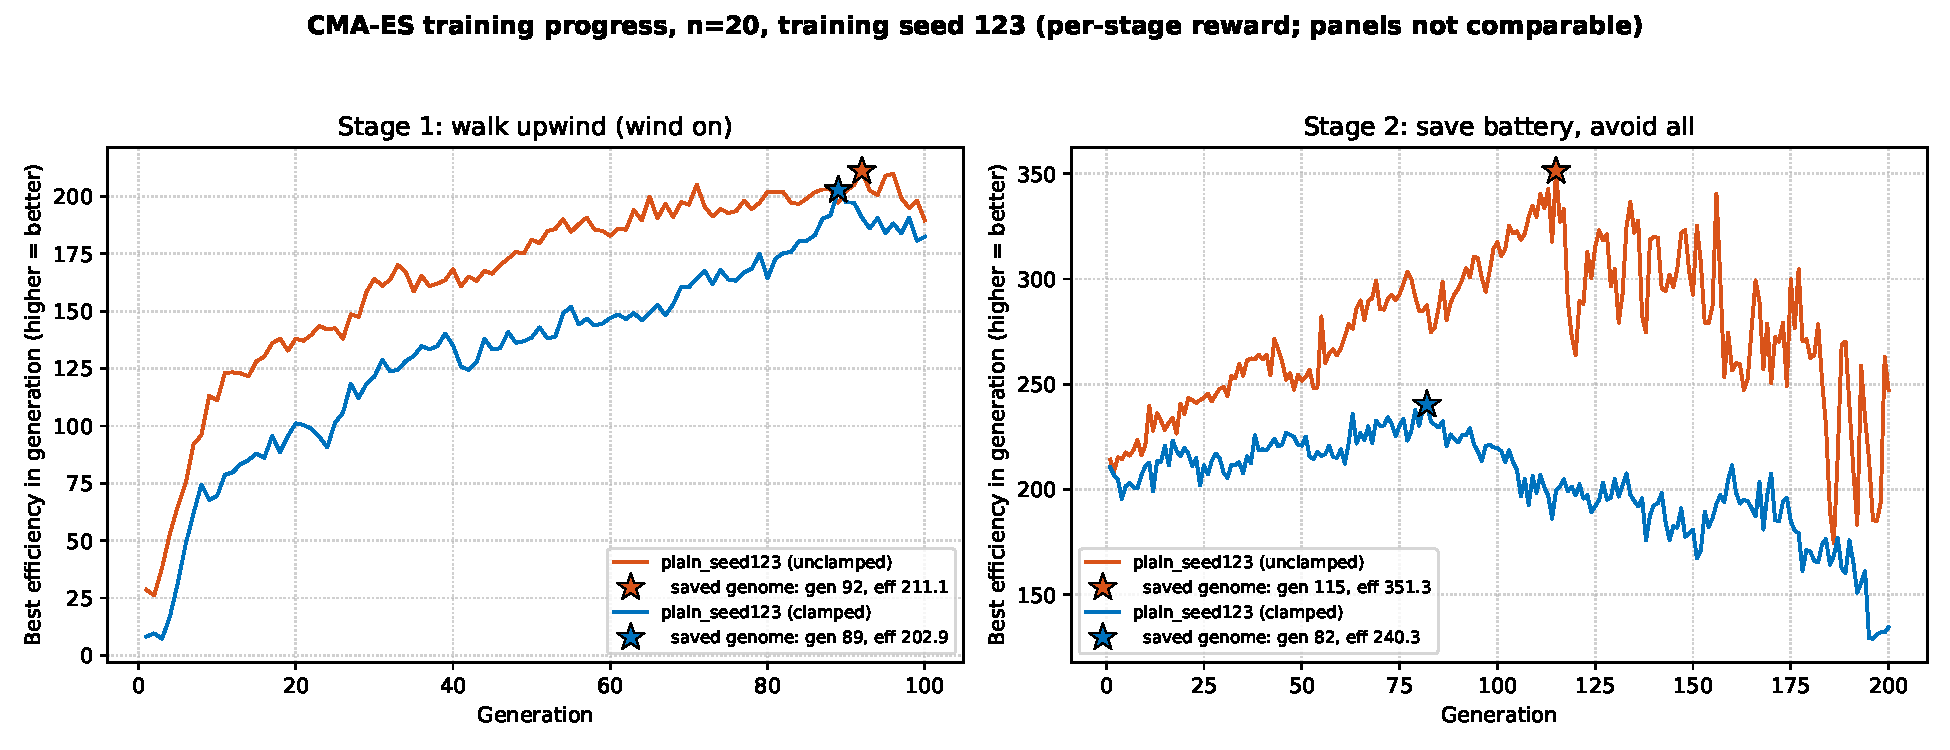
\includegraphics[width=\linewidth]{figures/fitness_curves_plain_seed123}
    \caption[]{\rev{Fitness evolution during the two evolutionary stages: fitness of the best candidate in each generation, for the controller evolved without (orange) and with (blue) the safety mechanisms. Each stage has its own fitness function, so the two panels are not comparable. Stars mark the best candidate ever evaluated, which is the result of the stage.}}
    \label{fig:fitness}
\end{figure}


\begin{table}[t]
  \centering
  \caption{Simulation parameters for the baseline controller.}
  \label{tab:baseline_params}
  \begin{tabular}{@{}lll@{}}
    \toprule
    \textbf{Parameter} & \textbf{Description} & \textbf{Value} \\
    \midrule
    $K_{1}$     & MDMC linear gain                           & $0.05~\text{m/s}$ \\
    $K_{2}$     & MDMC angular gain                          & $0.5~\text{rad/s}$ \\
    $\alpha$    & Steepness of potential function            & $2$ \\
    $\epsilon$  & Strength of potential function             & $1$ \\
    $d_{\text{des}}$ & Desired inter–robot distance         & $0.7~\text{m}$ \\
    $D_{\text{p}}$       & Max. interaction range (proximal control)  & $3~\text{m}$ \\
    $K_{\text{goal}}$  & Goal seeking weight                        & $3$ \\
    \rev{$B_0$} & \rev{Starting battery} & \rev{$150$} \\
    \bottomrule
  \end{tabular}
\end{table}


\begin{figure}[t]
  \centering
  \subfloat[\label{fig:scatter_batt_dist}]{
    \begin{minipage}[t]{0.55\textwidth}
      \centering
      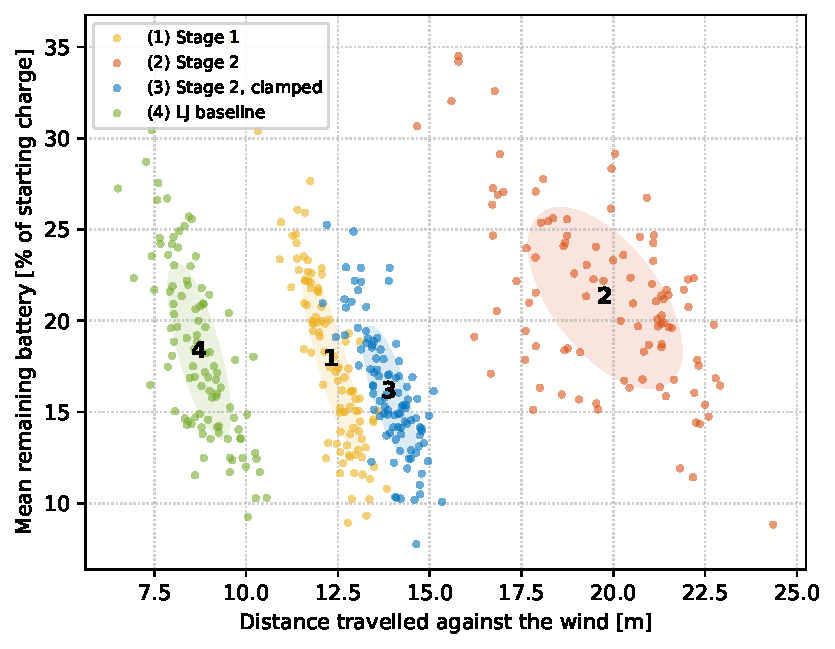
\includegraphics[width=0.98\linewidth]{figures/paper_dist_vs_battery_n20}
    \end{minipage}
  }
  \subfloat[\label{fig:boxplot}]{
    \begin{minipage}[t]{0.40\textwidth}
     \centering
      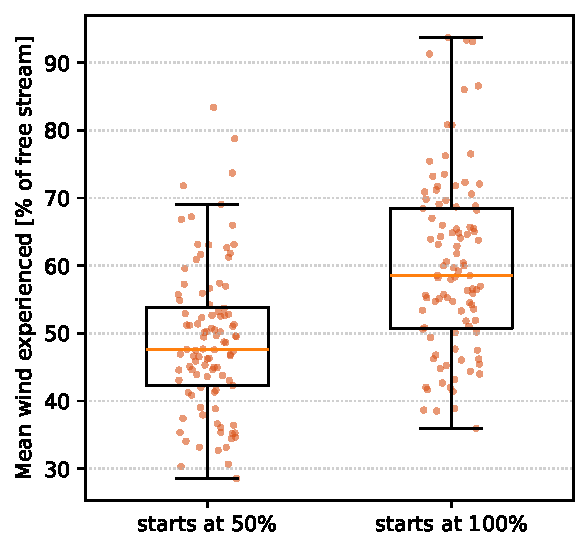
\includegraphics[width=0.95\linewidth]{figures/paper_battery_awareness_boxplot}
    \end{minipage}
  }
\caption{(a) Travelled distance against remaining battery of 100 simulations \rev{of 20 robots with the best controller of stage 1 (1), stage 2 (2), stage 2 evolved with the safety mechanisms (3), and the baseline (4); ellipses show one standard deviation.} Qualitative comparisons of all stages are provided in the supplementary video \cite{mahdavi_nasab_2026_ants}. (b) Wind speed experienced by the agents initialized at 50\% (left), and 100\% (right) over 100 simulations.}
  \label{fig:joined_scatter_box}
\end{figure}


\begin{table}[t]
\centering
\caption{\rev{Performance over 100 simulations of 20 robots (mean $\pm$ standard deviation). ``Both better'' counts the runs in which a controller travels further \emph{and} keeps more battery than the baseline on the same starting configuration. Differences from the baseline are tested with a two-sided Mann--Whitney U test: distance $p < 10^{-33}$ for all three controllers; battery $p = 3.3\times10^{-5}$ (stage 2, higher), $p = 0.002$ (stage 2 with safety mechanisms, lower) and $p = 0.49$ (stage 1, no difference).}}
\label{tab:results_main}
{\color{red}
\begin{tabular}{lccc}
\toprule
\textbf{Controller} & \textbf{Distance [m]} & \textbf{Battery [\%]} & \textbf{Both better} \\
\midrule
Stage 1 & $12.32 \pm 0.74$ & $17.87 \pm 4.87$ & 42/100 \\
Stage 2 & $19.78 \pm 2.05$ & $21.25 \pm 4.85$ & 69/100 \\
Stage 2, safety mechanisms & $13.90 \pm 0.67$ & $16.11 \pm 3.49$ & 37/100 \\
Baseline & $8.73 \pm 0.82$ & $18.31 \pm 4.70$ & -- \\
\bottomrule
\end{tabular}}
\end{table}


\begin{table}[t]
\centering
\caption{Results of battery awareness experiment (\rev{$p=5.0\times10^{-10}$}, $df=198$)}
\begin{tabular}{lccc}
\toprule
\textbf{Experiment} & \textbf{No. of runs} & \textbf{Mean} & \textbf{Standard deviation} \\
\midrule
Agent with 100\% battery & 100 & \rev{60.0} & \rev{13.0} \\
Agent with 50\% battery & 100 & \rev{49.0} & \rev{10.8} \\
\bottomrule
\end{tabular}
\label{tab:results_batt_aware}
\end{table}


\section{Experimental Results}
\label{sec:Exp:Results}

The fitness progression of the evolution of the ABCD-rules on a swarm of 20 agents across 300 generations (\rev{100 in stage 1 and 200 in stage 2}, as described in Section~\ref{sec:stages}) is depicted in Fig.~\ref{fig:fitness}. \rev{In stage 2 the best fitness peaks after 115 generations without the safety mechanisms and after 82 generations with them, and declines afterwards. Because we keep the best candidate ever evaluated, the resulting controllers come from these peaks.} After evolution, we evaluate the best controller obtained after each evolutionary stage and compare it with the standard collective motion baseline~\cite{article}. The baseline is implemented using only proximal control and goal-seeking terms. The parameters are reported in Table~\ref{tab:baseline_params}. \rev{The baseline runs in the same simulator, with the same wind, drag and battery model and the same starting configurations. Its robots start with 150 battery units, the native scale of the baseline model, rather than 100. Since the drain per step is the same, they start with $1.5\times$ as much energy; all battery values are reported as a percentage of each controller's own starting charge.}

Each controller is evaluated over 100 simulation runs of a swarm of 20 robots, initialized with random positions and random network weights; each simulation terminates when the battery of any robot is depleted. Performance is measured as the distance travelled to the left at termination and the average remaining battery across the swarm. \rev{None of the evaluation runs uses a starting configuration seen during evolution.}

Fig.~\ref{fig:scatter_batt_dist} \rev{and Table~\ref{tab:results_main}} summarize the main results. Each point corresponds to one simulation of the best controller from stage 1 (cluster 1), stage 2 (cluster 2), \rev{stage 2 evolved with the safety mechanisms (cluster 3)}, or the baseline (cluster 4), plotted in terms of distance travelled versus the average battery level of the swarm members at the end of the simulation. \rev{Because stage 1 already trains with the wind on and rewards progress against it, the stage-1 controller already travels further than the baseline ($12.3$ vs.\ $8.7$\,m) while keeping a similar amount of battery. Stage 2, which additionally rewards remaining battery and penalises collisions, travels $19.8$\,m, $127\%$ further than the baseline, while also keeping more battery ($21.3\%$ vs.\ $18.3\%$). Both differences are significant (Mann--Whitney U, $p < 10^{-33}$ for distance and $p = 3.3\times10^{-5}$ for battery), and it beats the baseline on both measures at once in 69 of the 100 runs. The controller evolved with the safety mechanisms trades part of this gain for collision safety: it travels $13.9$\,m ($59\%$ further than the baseline) but keeps significantly less battery ($16.1\%$, $p = 0.002$), and beats the baseline on both measures in 37 of the 100 runs.}

\rev{\textbf{Swarm size.} The advantage over the baseline depends strongly on the number of robots (Fig.~\ref{fig:swarm_size}). The baseline covers about 25\,m with up to 8 robots, but its distance falls steadily as the swarm grows, to 8.8\,m at 20 robots. The stage-2 controller behaves the other way round: a single robot covers only about 1\,m, and the distance grows with the swarm size to about 20\,m. The controller overtakes the baseline in distance at 12 robots (at 14 with the safety mechanisms). With 12 or fewer robots it never beats the baseline on distance and battery at the same time in any of 30 runs per swarm size. With 13 robots it does so in 2 of 30 runs, and with 20 robots in 23 of 30. The controllers were evolved with 20 robots only, and they do not transfer to small swarms. Part of the advantage at 20 robots also reflects the baseline getting worse in large swarms: its parameters (Table~\ref{tab:baseline_params}) are those of~\cite{article} and were not tuned for 20 robots, so the $127\%$ gain is measured against a baseline at its weakest swarm size in this range.}

We argue that the strategies learned in \rev{stage 2} rely primarily on local inter-robot interactions rather than the compass information. We contrast the controllers of stages 1 and \rev{2} by testing them with 1 and 5 agents \rev{(Fig.~\ref{fig:Debunk_Compass})}. \rev{The stage-1 controller heads upwind whether it is alone or in a group: a single robot travels about 14\,m, heading straight for the wall and then following it upwind (Fig.~\ref{fig:Debunk_Compass}, top left), and five robots move upwind spread out, each on its own path. The stage-2 controller behaves very differently alone and in a group. A single robot turns in continuous circles and drifts only about a metre (top right), whereas five robots stay together, move upwind and repeatedly loop around one another, changing positions within the group (bottom right). The stage-2 controller therefore depends on its neighbours to make progress at all: its behaviour is collective, arising from local interactions rather than from the compass alone.}

So far, we have shown that the evolved controller achieves energy-efficient flocking with an emergent formation reconfiguration strategy and improved distance-battery trade-offs. However, these results alone do not reveal whether the controller actually exploits the internal battery state. To test whether battery awareness has any impact on the strategy that robots adopt, we compare the behaviour of an agent initialised normally with $100\%$ battery to an agent initialised with $50\%$ battery at the beginning of the simulation. The percentage wind speed of the grid cells where the agent travels, $U_{i,j}^\%$, is averaged over the simulation time. This parameter is chosen to quantify conservativeness; an agent that drives a lot in the front of the swarm will expose itself to much higher average $U_{i,j}^\%$ than an agent that tries to stay in the middle of the swarm shielded by others. Once again, we note that the robots do not have any onboard sensors for wind measurement. We ran 100 simulations with all agents initialized at full charge (100\%) and recorded the average $U_{i,j}^\%$ along the trajectory of a representative agent. We then repeated the experiment, but this time with one agent initialized at half charge (50\%) while all others remained at 100\%. As shown in Fig.~\ref{fig:boxplot} and Table \ref{tab:results_batt_aware}, the mean $U_{i,j}^\%$ for a normal agent was \rev{60.0\%}, whereas an agent initialized with reduced battery travelled through regions with a lower mean $U_{i,j}^\%$ of \rev{49.0\%}. A t-test confirmed the statistical significance of this difference (\rev{$t = 6.54$, $p=5.0\times10^{-10}$}, $df=198$). \rev{Because a simulation ends when any battery is empty, runs with the half-charged agent are shorter (141\,s vs.\ 169\,s on average), so the two averages cover episodes of different length.} With this, we conclude that battery monitoring helps agents find adaptive strategies to increase the swarm's endurance.

\subsection{\texorpdfstring{\rev{Leadership and Position Changes}}{Leadership and Position Changes}}
\label{sec:leadership_results}
\begingroup\color{red}
We compute the metrics of Section~\ref{sec:metrics} over 30 simulations of 20 robots for each
controller (Table~\ref{tab:leadership}, Fig.~\ref{fig:leadership}). The stage-2 controller
changes its front robot about 10 times per minute, almost five times as often as the baseline
(2.1 per minute); with the safety mechanisms it does so 4.8 times per minute. Each of these
changes lasts at least 1.5\,s, so different robots genuinely take the exposed front position
in turn (Fig.~\ref{fig:leadership}a). The raw count of front changes gives the opposite
impression: the baseline's front robot changes almost 600 times per simulation, but only
about 2\% of those changes persist, because its robots move nearly level with each other and
the front identity flickers between them. For the stage-2 controller, 65\% of the raw changes
persist. For the same reason, front occupancy does not separate the controllers at 20 robots
(0.84 for stage 2 against 0.89 for the baseline): the flickering spreads the baseline's front
time over many robots. With 10 robots, where the baseline flickers less, the difference is
clear (0.90 against 0.26).

The rotation is not balanced in the sense of Voelkl et al.~\cite{voelkl2015}. The
reciprocity between front and back time is negative for both evolved controllers ($-0.26$
and $-0.19$), whereas it is close to zero for the baseline ($0.07$). Robots that spend more
time at the front spend less time at the back, so over a whole simulation some robots stay
towards the front and others towards the back, even though the front itself changes hands
frequently. None of the controllers shows a strong turning hierarchy: the leadership entropy
is at least 0.97 for all three, and the evolved controllers' hierarchies are only slightly
steeper than the baseline's (0.63 and 0.62 against 0.55). The evolved behaviour is therefore
best described as frequent exchange of the front position without fixed leaders, rather than
as a strict rotation through all positions.
\endgroup

\begin{table}[t]
\centering
\caption{\rev{Leadership metrics for 20 robots, median [interquartile range] over 30 simulations. All differences from the baseline are significant (Mann--Whitney U, $p < 0.004$).}}
\label{tab:leadership}
{\color{red}
\begin{tabular}{lccc}
\toprule
\textbf{Metric} & \textbf{Stage 2} & \textbf{Stage 2, clamped} & \textbf{Baseline} \\
\midrule
Front changes per minute & 9.9 [9.5, 10.2] & 4.8 [3.5, 5.6] & 2.1 [1.7, 2.5] \\
Raw changes that persist [\%] & 65 [57, 68] & 38 [32, 45] & 2.1 [1.8, 2.6] \\
Front occupancy entropy & 0.84 [0.81, 0.88] & 0.42 [0.36, 0.51] & 0.89 [0.88, 0.91] \\
Reciprocity $r$ & $-0.26$ [$-0.34$, $-0.21$] & $-0.19$ [$-0.23$, $-0.14$] & 0.07 [$-0.04$, 0.19] \\
Hierarchy entropy & 0.98 [0.97, 0.98] & 0.98 [0.98, 0.99] & 0.99 [0.99, 0.99] \\
Hierarchy steepness & 0.63 [0.55, 0.69] & 0.62 [0.54, 0.67] & 0.55 [0.50, 0.59] \\
\bottomrule
\end{tabular}}
\end{table}

\begin{figure}[t]
  \centering
  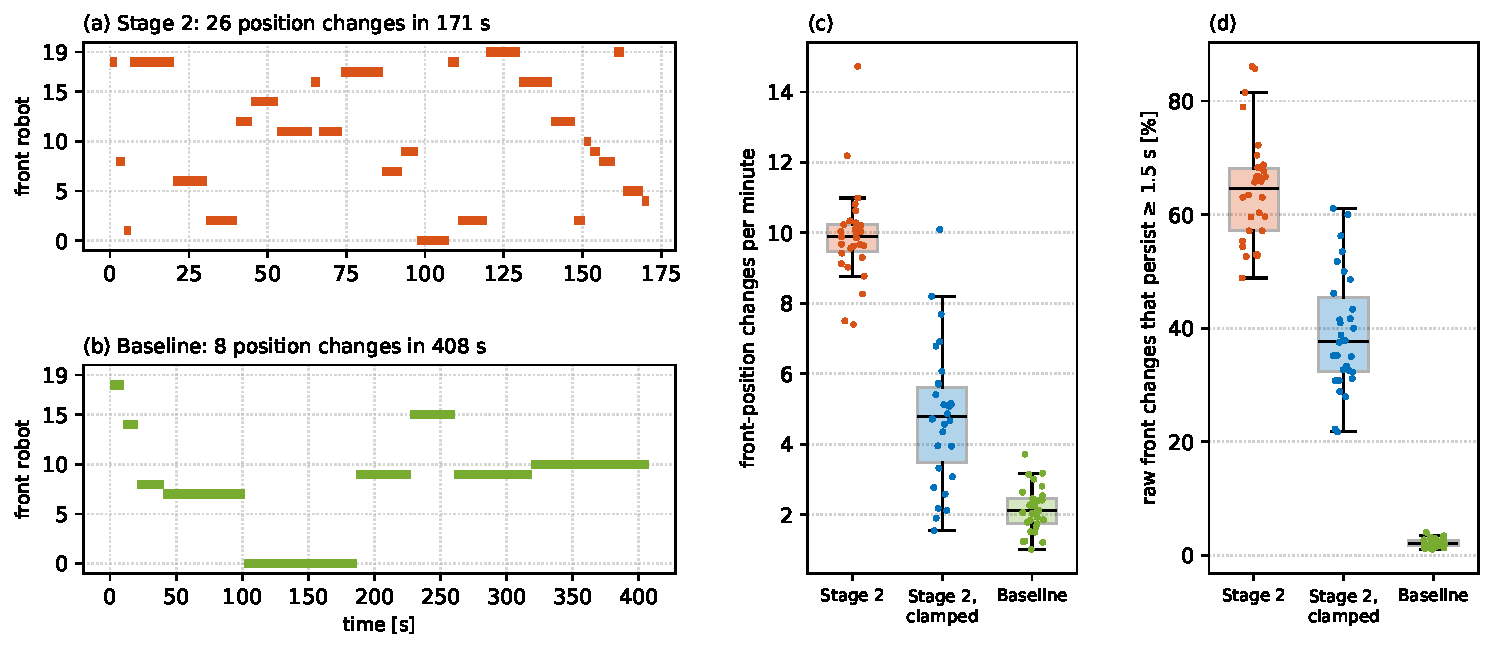
\includegraphics[width=\linewidth]{figures/paper_leadership_n20}
  \caption{\rev{Front-position changes with 20 robots. (a, b) Which robot is at the front over time in one simulation, after discarding spells shorter than 1.5\,s, for the stage-2 controller and the baseline; note the different time axes. (c) Front-position changes per minute and (d) share of raw front changes that persist for at least 1.5\,s, over 30 simulations per controller.}}
  \label{fig:leadership}
\end{figure}

\subsection{\texorpdfstring{\rev{Real-Robot Experiments}}{Real-Robot Experiments}}
\label{sec:hardware_results}
\rev{In simulation, the controller does not outperform the baseline in swarms as small as those we can run on real robots (Fig.~\ref{fig:swarm_size}). The real-robot experiments therefore test whether the evolved controller transfers from simulation to hardware, not whether it beats the baseline.}

\begingroup\color{red}
We ran 30 trials of five robots for both Stage~2 and Stage~2 with the safety mechanisms, in a $3.5\,\text{m}\times 6\,\text{m}$ arena, well below the $10\,\text{m}\times 10\,\text{m}$ arena the controllers were evolved in. OptiTrack tracking of individual robots is intermittent at this range and drops out for extended periods when robots are close together, so we restrict the leadership metrics of Section~\ref{sec:metrics} to the longest window in each trial during which all five robots are tracked without interruption (at least 10\,s); this leaves 28 of 30 trials for Stage~2 and 19 of 30 for Stage~2 with the safety mechanisms. Minimum inter-robot distances recorded by OptiTrack are frequently smaller than the robots' own diameter, which is physically impossible; this reflects tracking bias at close range rather than genuine collisions, none of which were observed. Unlike simulation, where an episode ends once any robot's battery is depleted, each real trial runs for a fixed duration of approximately 98\,s regardless of battery state; the virtual battery drains smoothly over this time (from full charge to $77\%$ and $75\%$ remaining on average for Stage~2 with and without the safety mechanisms respectively, never depleting), confirming the online model of Section~\ref{sec:hardware_setup} produces plausible drainage from real tracked motion, but the real trials are consequently too short to say anything about the battery-depletion endpoint simulation results are measured at.

Table~\ref{tab:leadership_hardware} and Figs.~\ref{fig:hardware_traj_stage2}--\ref{fig:hardware_leadership_stage2_clamped} compare the real trajectories against a simulation of the same controller and swarm size. The core result of Section~\ref{sec:leadership_results} replicates: the front position changes hands frequently for both controllers on real hardware (30.0 and 36.2 times per minute for Stage~2 with and without the safety mechanisms respectively), markedly more often than in simulation (19.5 and 7.2 changes per minute respectively), and front-occupancy and hierarchy entropy remain high, so no single robot dominates the front. We cannot fully separate a genuine increase in turn-taking frequency at this scale from OptiTrack position noise flipping the front rank more readily when robots are close together, which Section~\ref{sec:metrics}'s persistence filter only partly controls for; the same caveat applies to the reciprocity result below.

Two results differ from the simulated distribution. First, the reciprocity between front and back time is negative in simulation for both controllers (Table~\ref{tab:leadership_hardware}); on hardware it is clearly positive for Stage~2 (median $0.41$) and no longer distinguishable from zero for Stage~2 with the safety mechanisms (median $0.05$, interquartile range $[-0.24, 0.36]$ straddling zero). For Stage~2 at least, robots that spend more time at the front also spend more time at the back, rather than settling into separate front-leaning and back-leaning roles. \todo[inline]{Confirm this interpretation with more trials/seeds before final submission -- reciprocity is a 5-point correlation per trial.} Second, front-occupancy entropy reverses direction between the two controllers: for Stage~2 it is lower on hardware than in simulation ($0.76$ vs.\ $0.92$), but for Stage~2 with the safety mechanisms it is higher on hardware ($0.77$ vs.\ $0.54$) -- on the real robots, the safety-mechanism controller rotates the front position more evenly than its own simulated counterpart does. Hierarchy entropy and steepness, which appeared to differ substantially from hardware when we compared against a single archived simulation run, are in fact comparable once measured against the same 30-seed distribution as Table~\ref{tab:leadership} (Table~\ref{tab:leadership_hardware}): that single run was, in retrospect, atypically flat for both controllers. We also observe both controllers spending a substantial fraction of each trial near one of the arena's walls along $y$, more than in the much larger simulated arena: the wall clamp of Eq.~\ref{eq:clamp_real} engages far more often at this scale than its simulated counterpart does in the $10\,\text{m}\times 10\,\text{m}$ arena, and, like Eq.~\ref{eq:clamp}, it only reduces forward speed and does not alter heading, so a robot facing a wall can remain there for several seconds before turning away on its own. This is the same kind of change we earlier found does not work for the inter-robot clamp (Section~\ref{sec:safety}): a differently-calibrated clamp added at deployment without retraining. We did not retrain against the real arena's wall scale, so some of the discrepancies above -- particularly the wall-dwelling behaviour itself -- may reflect this mismatch rather than a property of the controller's learned strategy. Neither training nor deployment clamps speed along $x$ (Section~\ref{sec:safety}), and unlike the simulated arena this axis is not actually unbounded on the real robots, so a robot travelling far enough along it is only stopped by the physical wall.
\endgroup

\begin{table}[t]
\centering
\caption{\rev{Leadership metrics for five real robots, median [interquartile range]. Hardware columns are over the trials with a continuous fully-tracked window of at least 10\,s (28 of 30 for Stage~2, 19 of 30 for Stage~2 with the safety mechanisms). Simulation columns are the same swarm size and the same 30-seed sweep methodology as Table~\ref{tab:leadership}, run at $n=5$ rather than $n=20$.}}
\label{tab:leadership_hardware}
{\color{red}
\begin{tabular}{lcccc}
\toprule
 & \multicolumn{2}{c}{\textbf{Stage 2}} & \multicolumn{2}{c}{\textbf{Stage 2, clamped}} \\
\textbf{Metric} & \textbf{Hardware} & \textbf{Simulation} & \textbf{Hardware} & \textbf{Simulation} \\
\midrule
Front changes per minute & 36.2 [27.9, 43.1] & 19.5 [14.4, 24.1] & 30.0 [25.4, 37.7] & 7.2 [4.6, 11.4] \\
Raw changes that persist [\%] & 36 [32, 48] & 49 [44, 51] & 44 [30, 61] & 43 [34, 55] \\
Front occupancy entropy & 0.76 [0.63, 0.85] & 0.92 [0.86, 0.95] & 0.77 [0.61, 0.85] & 0.54 [0.41, 0.64] \\
Reciprocity $r$ & 0.41 [0.08, 0.67] & $-0.47$ [$-0.65$, $-0.29$] & 0.05 [$-0.24$, 0.36] & $-0.54$ [$-0.67$, $-0.33$] \\
Hierarchy entropy & 0.86 [0.81, 0.95] & 0.89 [0.81, 0.95] & 0.85 [0.82, 0.92] & 0.84 [0.78, 0.90] \\
Hierarchy steepness & 0.84 [0.70, 0.98] & 0.79 [0.64, 0.94] & 0.91 [0.79, 0.97] & 0.93 [0.81, 1.01] \\
\bottomrule
\end{tabular}}
\end{table}

\begin{figure}[t]
  \centering
  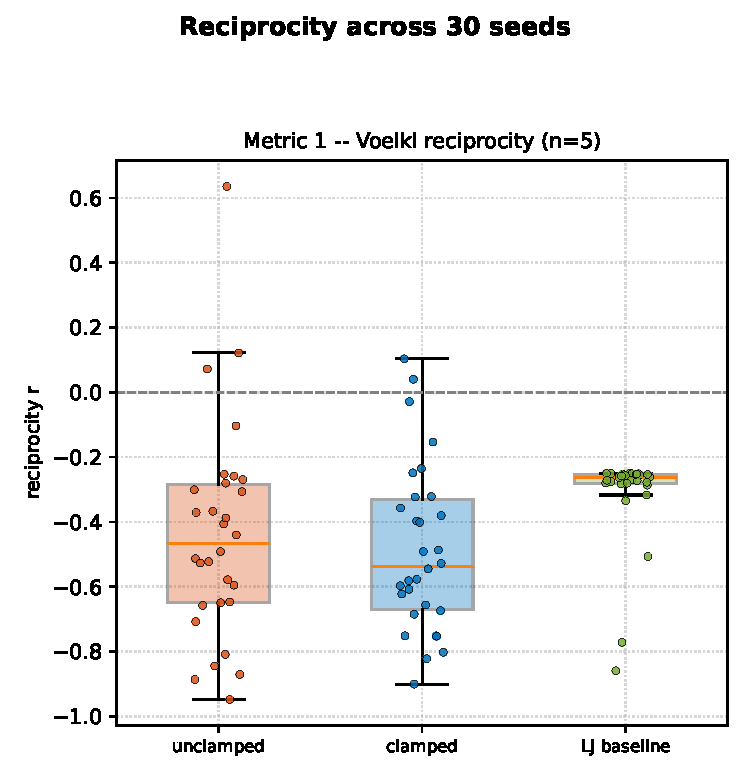
\includegraphics[width=\linewidth]{figures/metric1_seed_sweep_n5}
  \caption{\rev{Reciprocity $r$ (Table~\ref{tab:leadership_hardware}) across the same 30-seed sweep, $n=5$, for both real-robot controllers and the baseline; each point is one simulated seed. Compare against the hardware distribution of Fig.~\ref{fig:hardware_leadership_stage2}--\ref{fig:hardware_leadership_stage2_clamped}.}}
  \label{fig:sim_seed_sweep_reciprocity_n5}
\end{figure}

\begin{figure}[t]
  \centering
  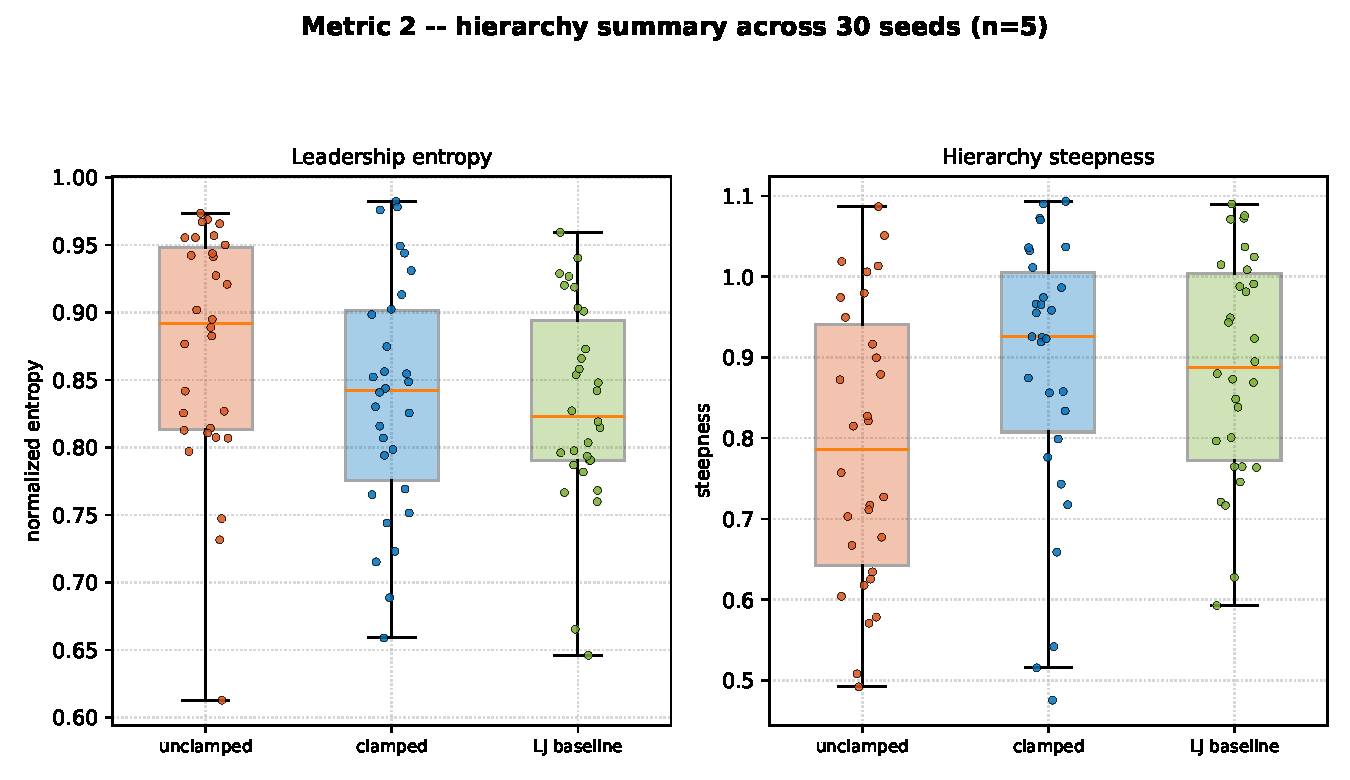
\includegraphics[width=\linewidth]{figures/metric2_seed_sweep_n5}
  \caption{\rev{Leadership entropy and hierarchy steepness (Table~\ref{tab:leadership_hardware}) across the same 30-seed sweep, $n=5$. Compare against the hardware distribution of Figs.~\ref{fig:hardware_leadership_stage2}--\ref{fig:hardware_leadership_stage2_clamped}: both quantities, which looked markedly different from hardware against the single archived seed, fall within the range shown here.}}
  \label{fig:sim_seed_sweep_hierarchy_n5}
\end{figure}

\begin{figure}[t]
  \centering
  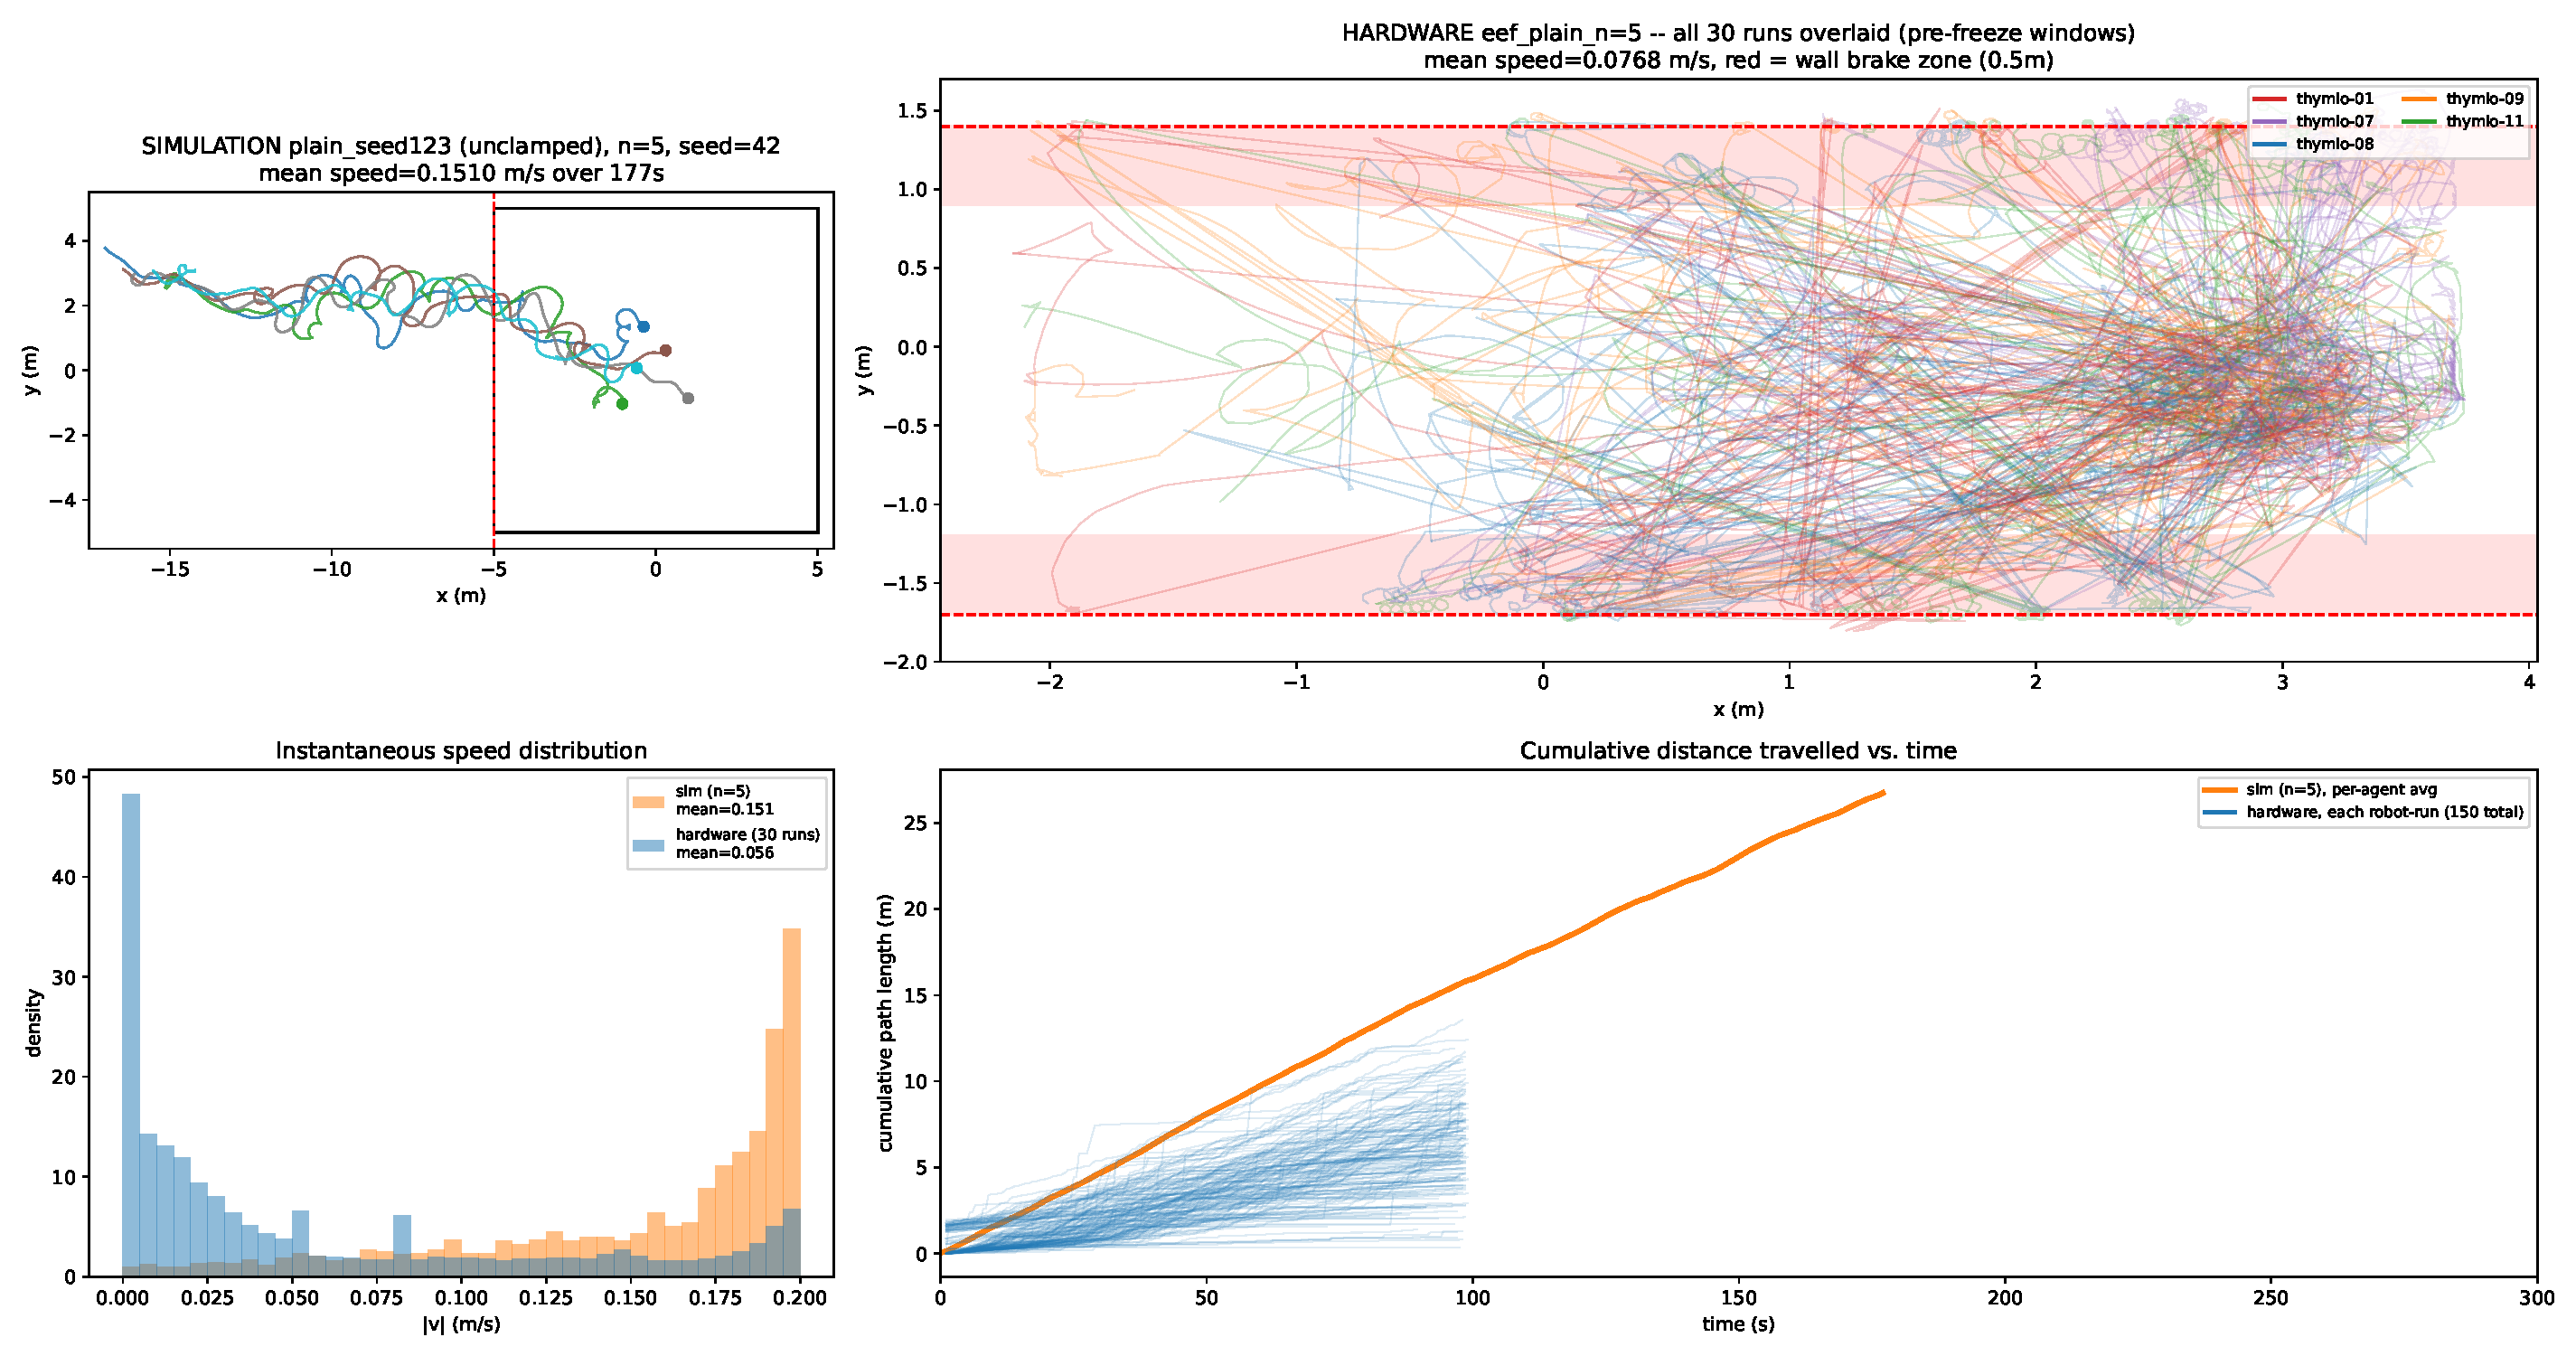
\includegraphics[width=\linewidth]{figures/hardware_trajectories_stage2}
  \caption{\rev{Stage 2: simulated trajectory (left, seed 42) against all 30 real trials overlaid (top right, each truncated to before any permanent tracking loss), instantaneous speed distribution (bottom left) and cumulative distance travelled (bottom right). Shaded bands mark the deployment-only speed-clamped zone near each wall.}}
  \label{fig:hardware_traj_stage2}
\end{figure}

\begin{figure}[t]
  \centering
  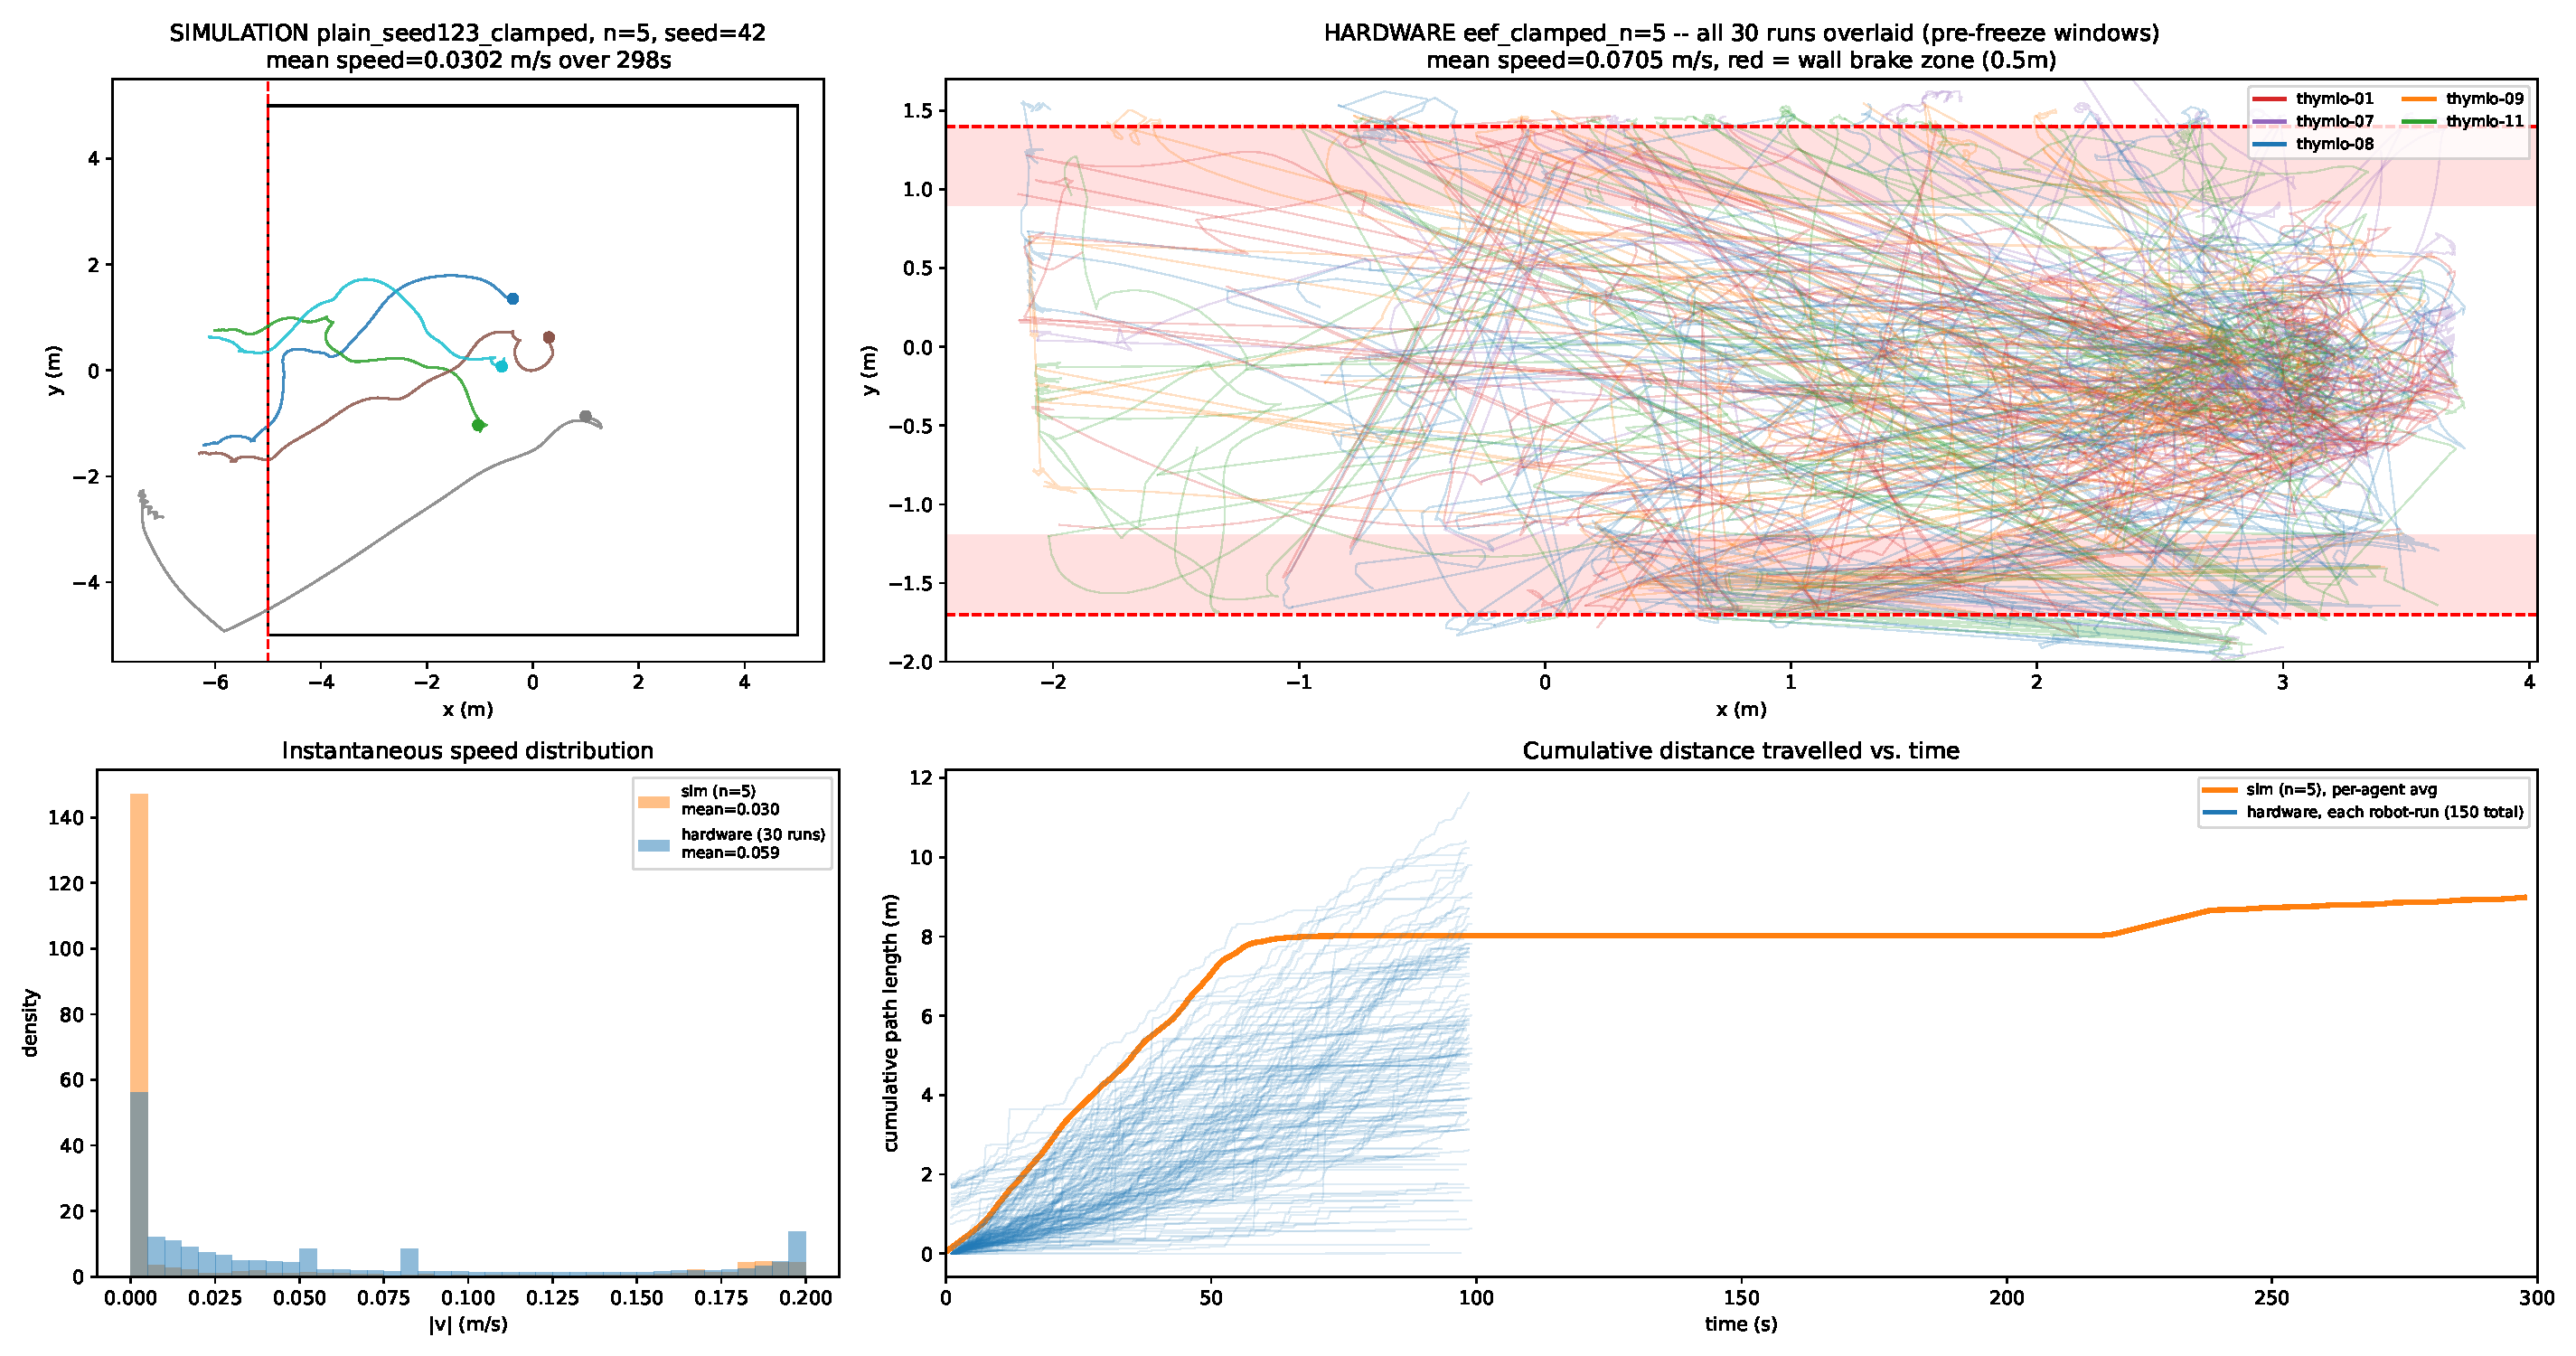
\includegraphics[width=\linewidth]{figures/hardware_trajectories_stage2_clamped}
  \caption{\rev{As Fig.~\ref{fig:hardware_traj_stage2}, for Stage 2 with the safety mechanisms -- the controller actually deployed on the robots.}}
  \label{fig:hardware_traj_stage2_clamped}
\end{figure}

\begin{figure}[t]
  \centering
  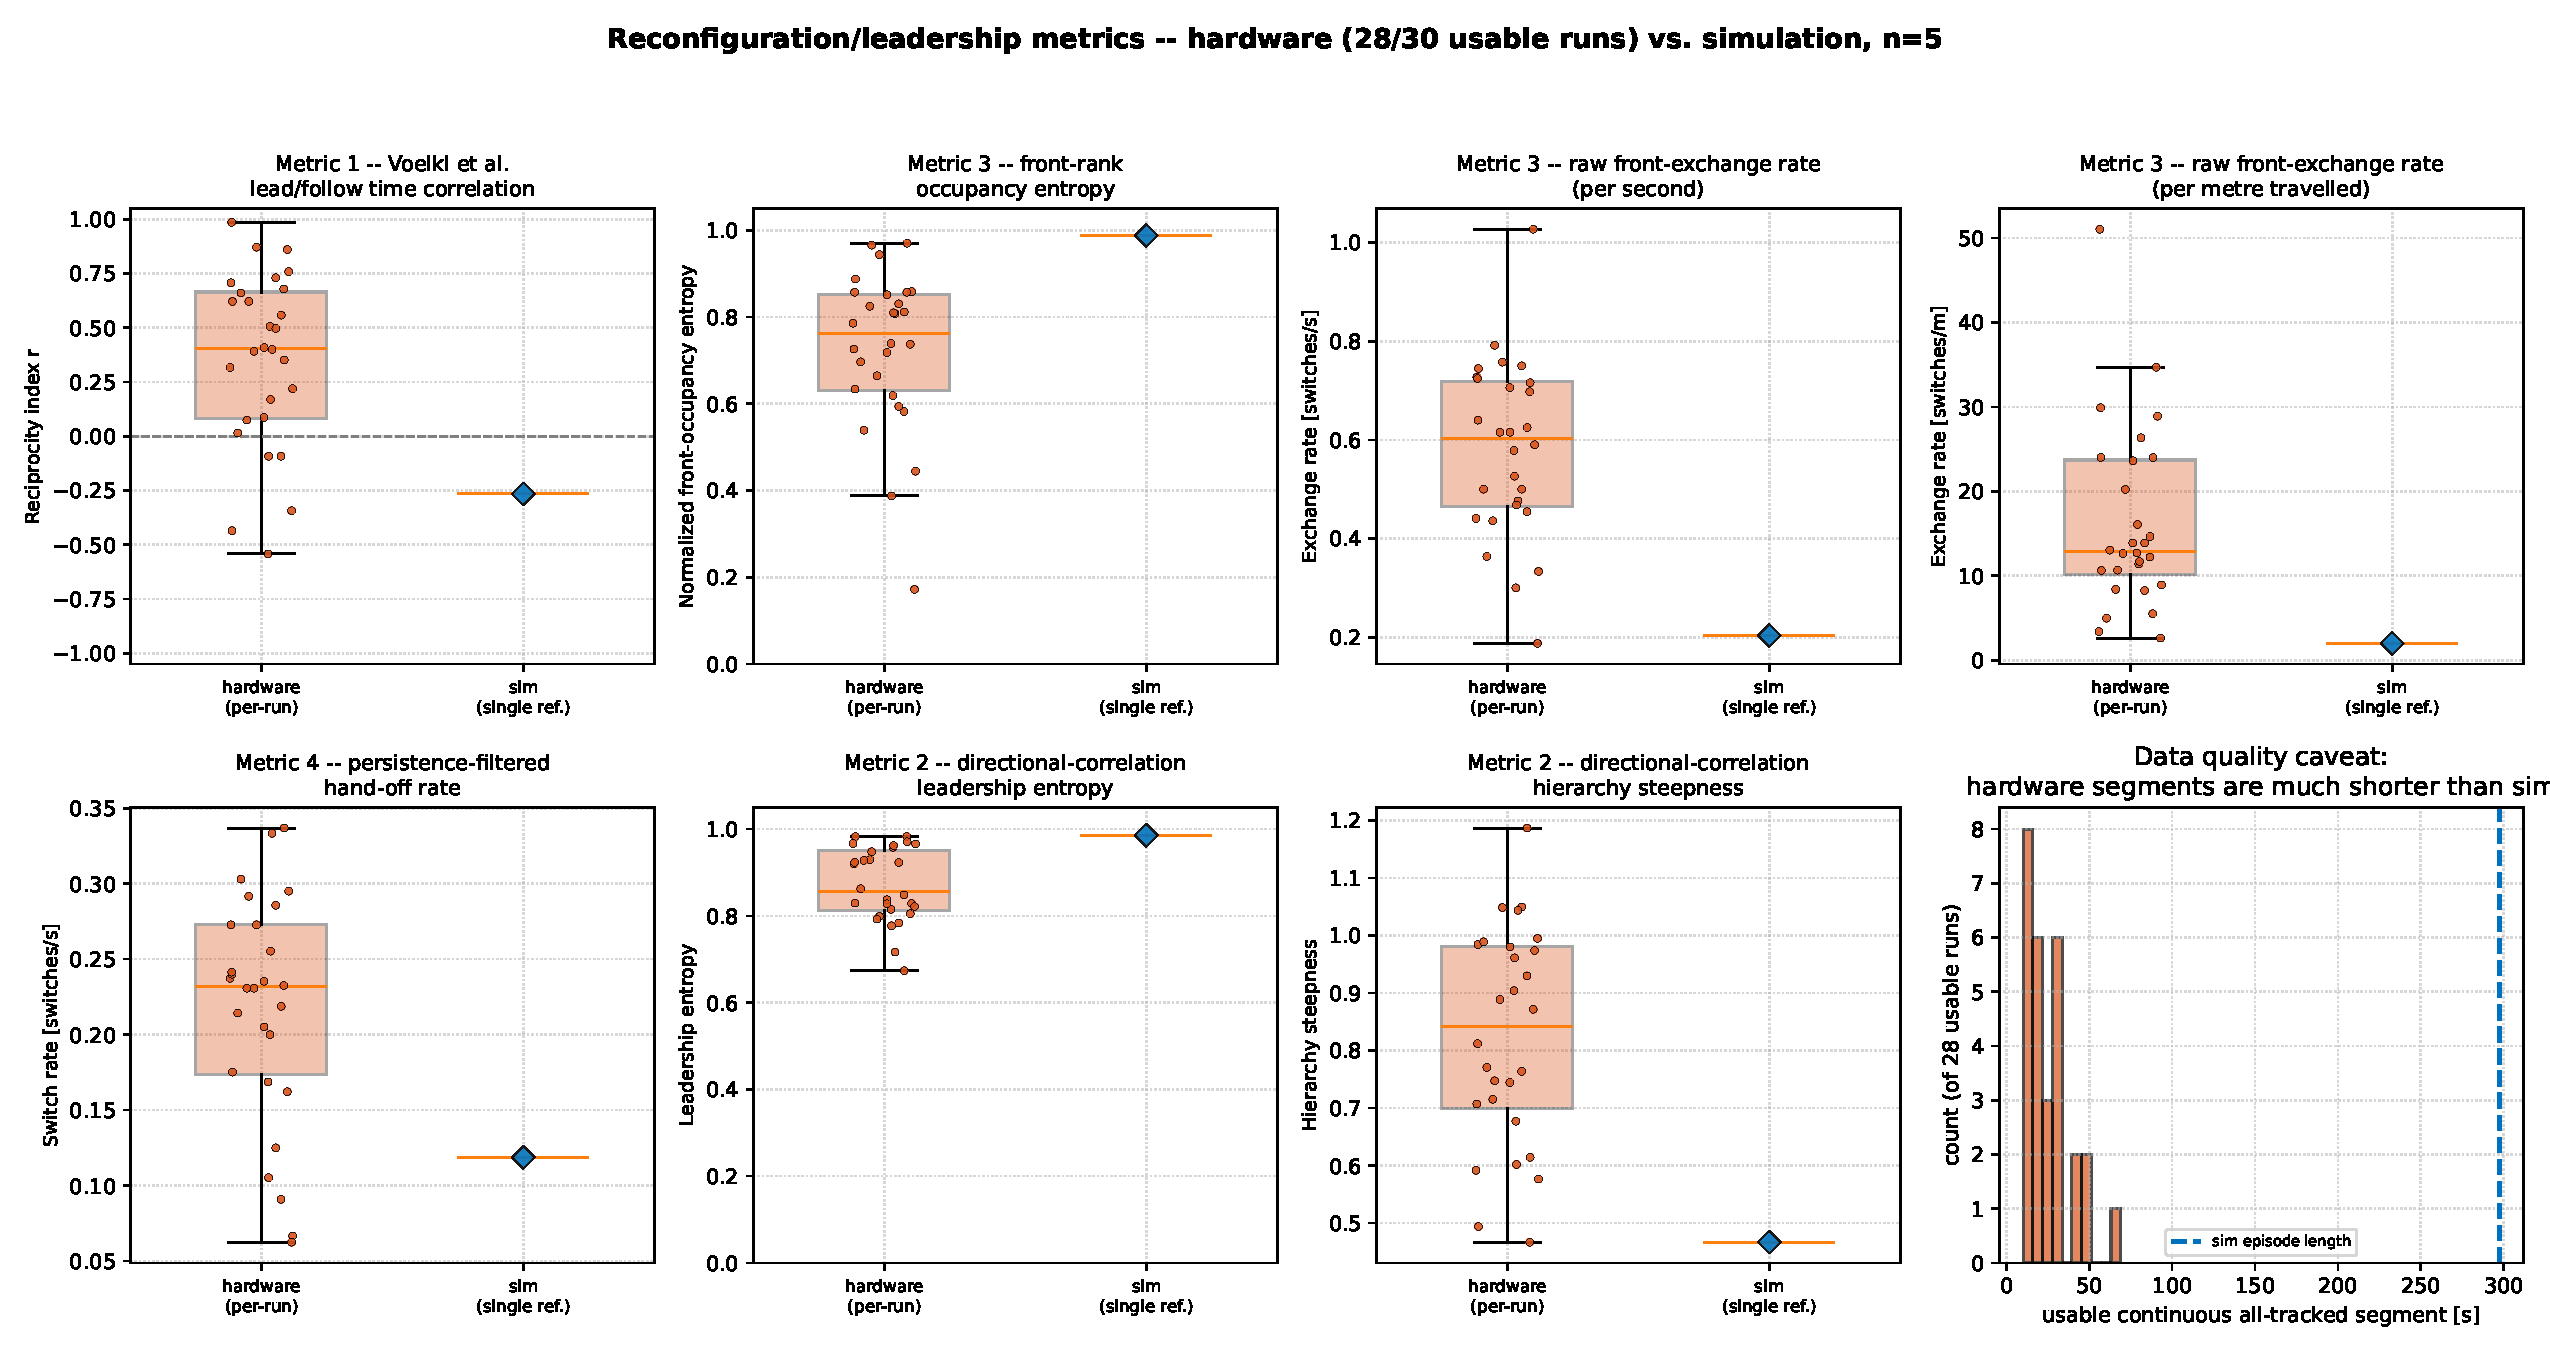
\includegraphics[width=\linewidth]{figures/hardware_leadership_stage2}
  \caption{\rev{Leadership metrics of Table~\ref{tab:leadership_hardware} for Stage 2: each real trial (orange) against the single matched simulation (blue diamond).}}
  \label{fig:hardware_leadership_stage2}
\end{figure}

\begin{figure}[t]
  \centering
  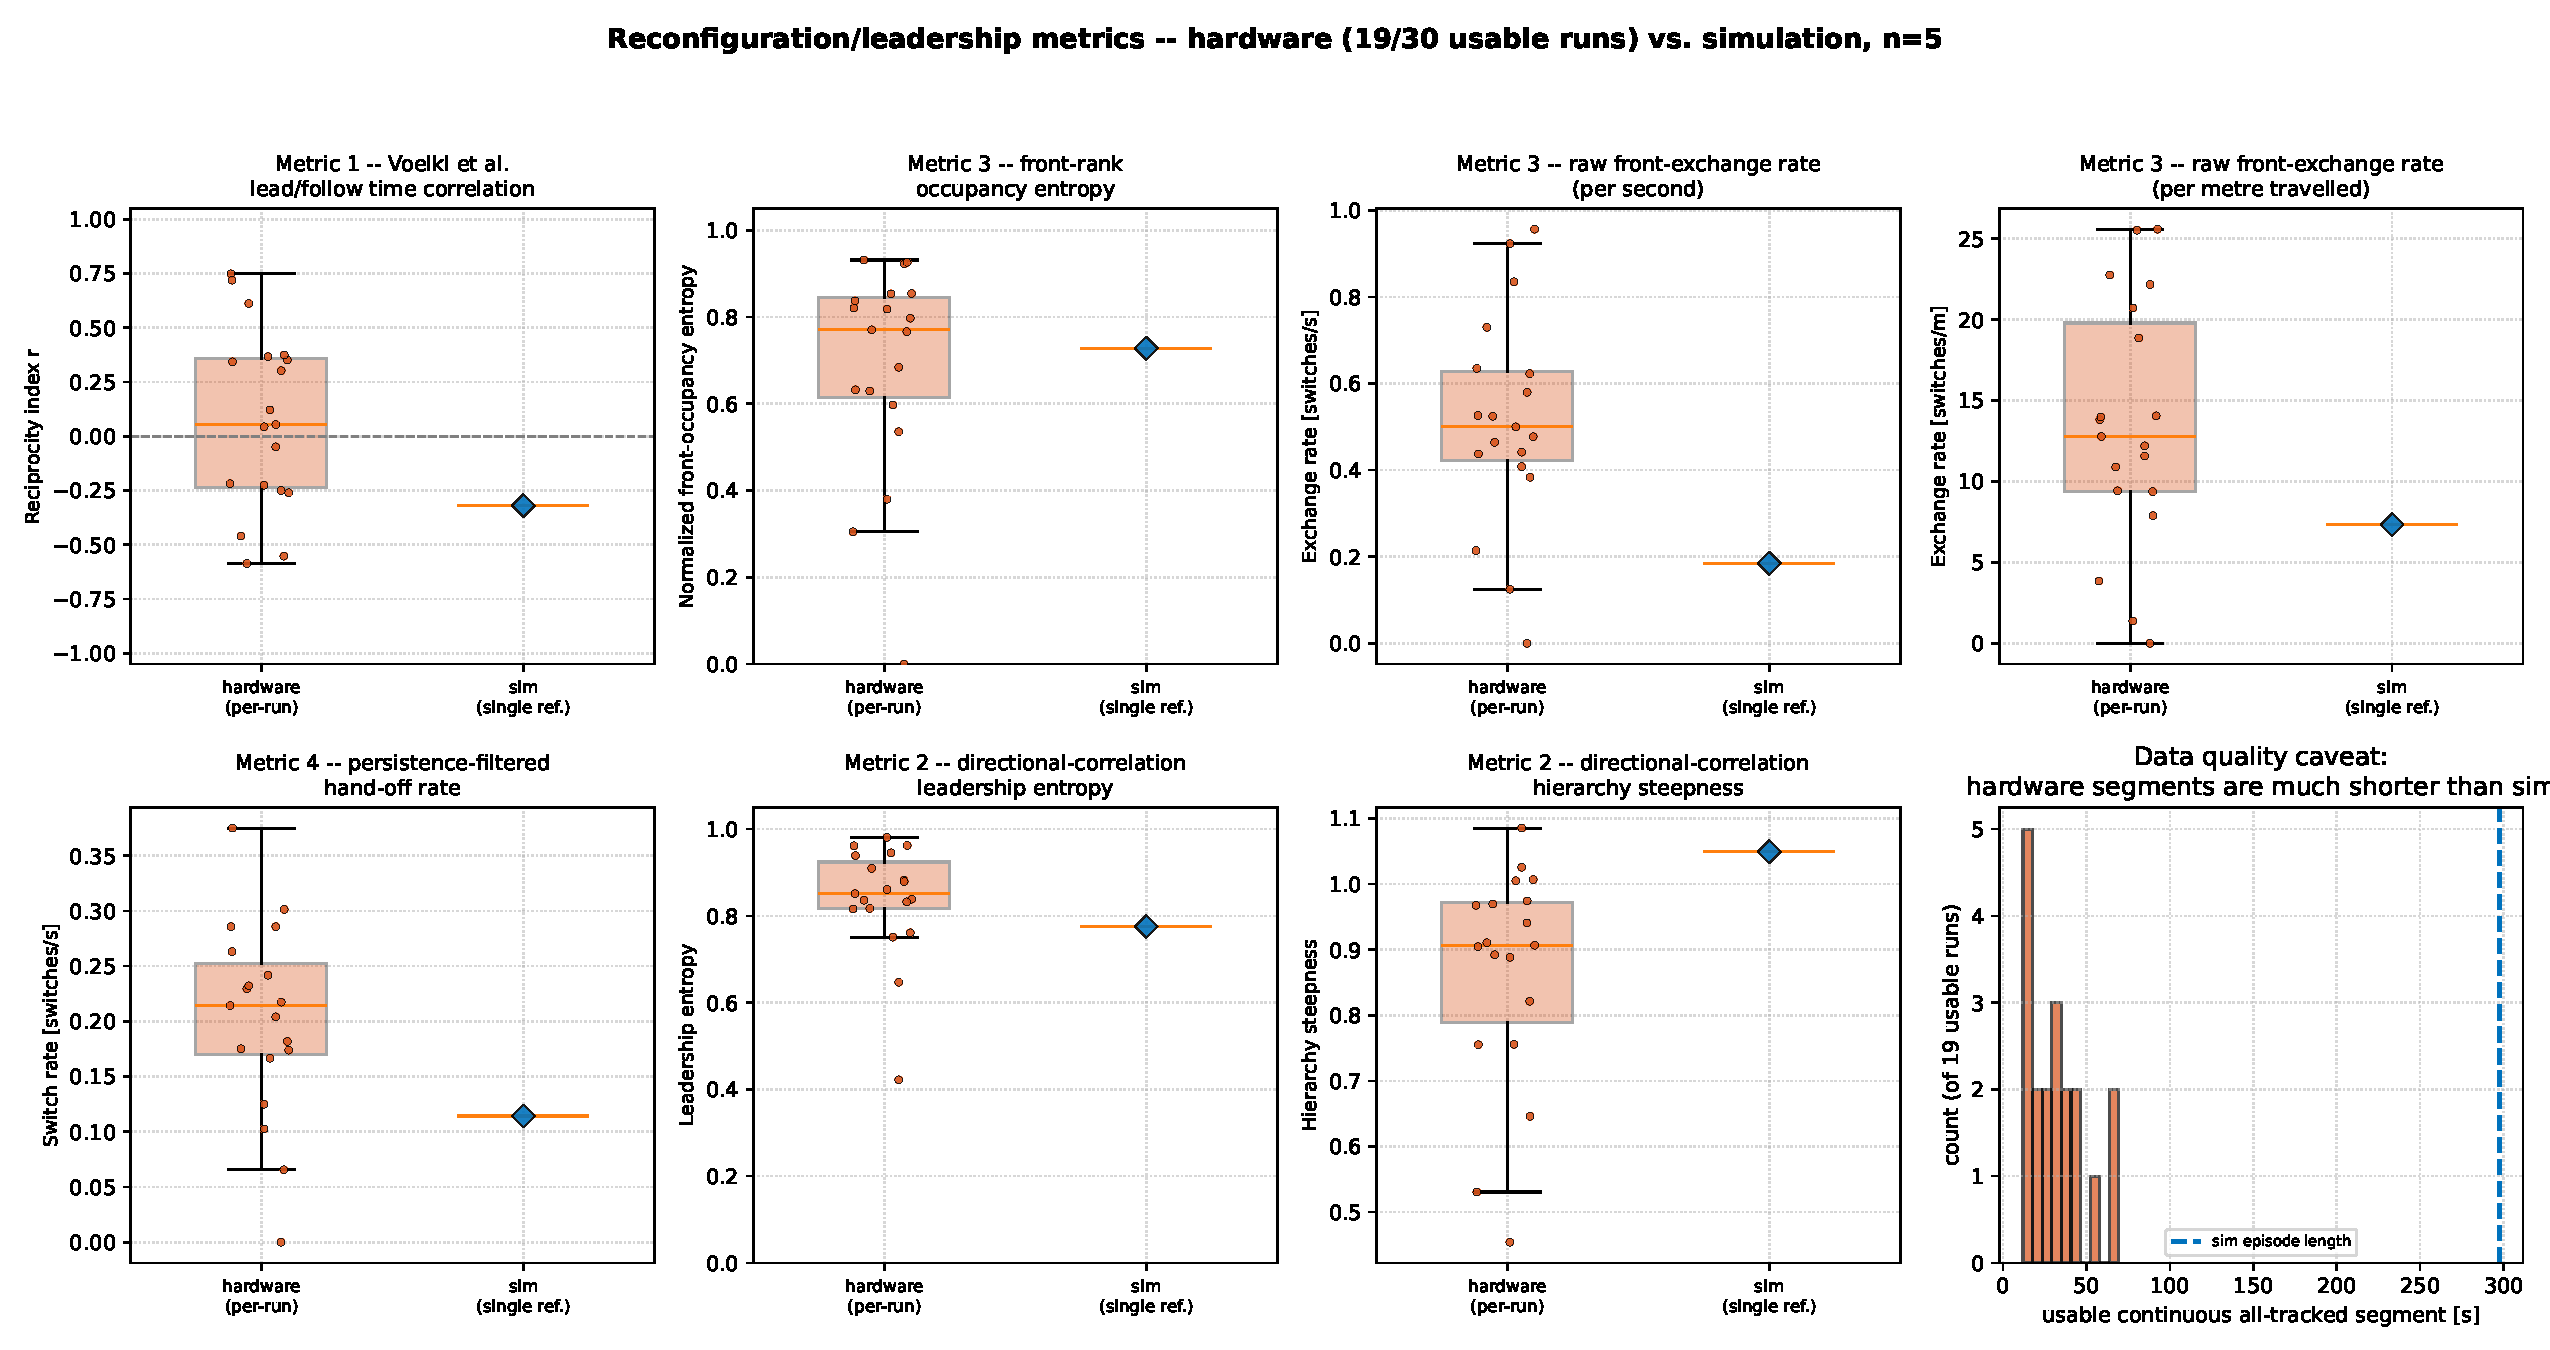
\includegraphics[width=\linewidth]{figures/hardware_leadership_stage2_clamped}
  \caption{\rev{As Fig.~\ref{fig:hardware_leadership_stage2}, for Stage 2 with the safety mechanisms.}}
  \label{fig:hardware_leadership_stage2_clamped}
\end{figure}


\begin{figure}[t]
  \centering
  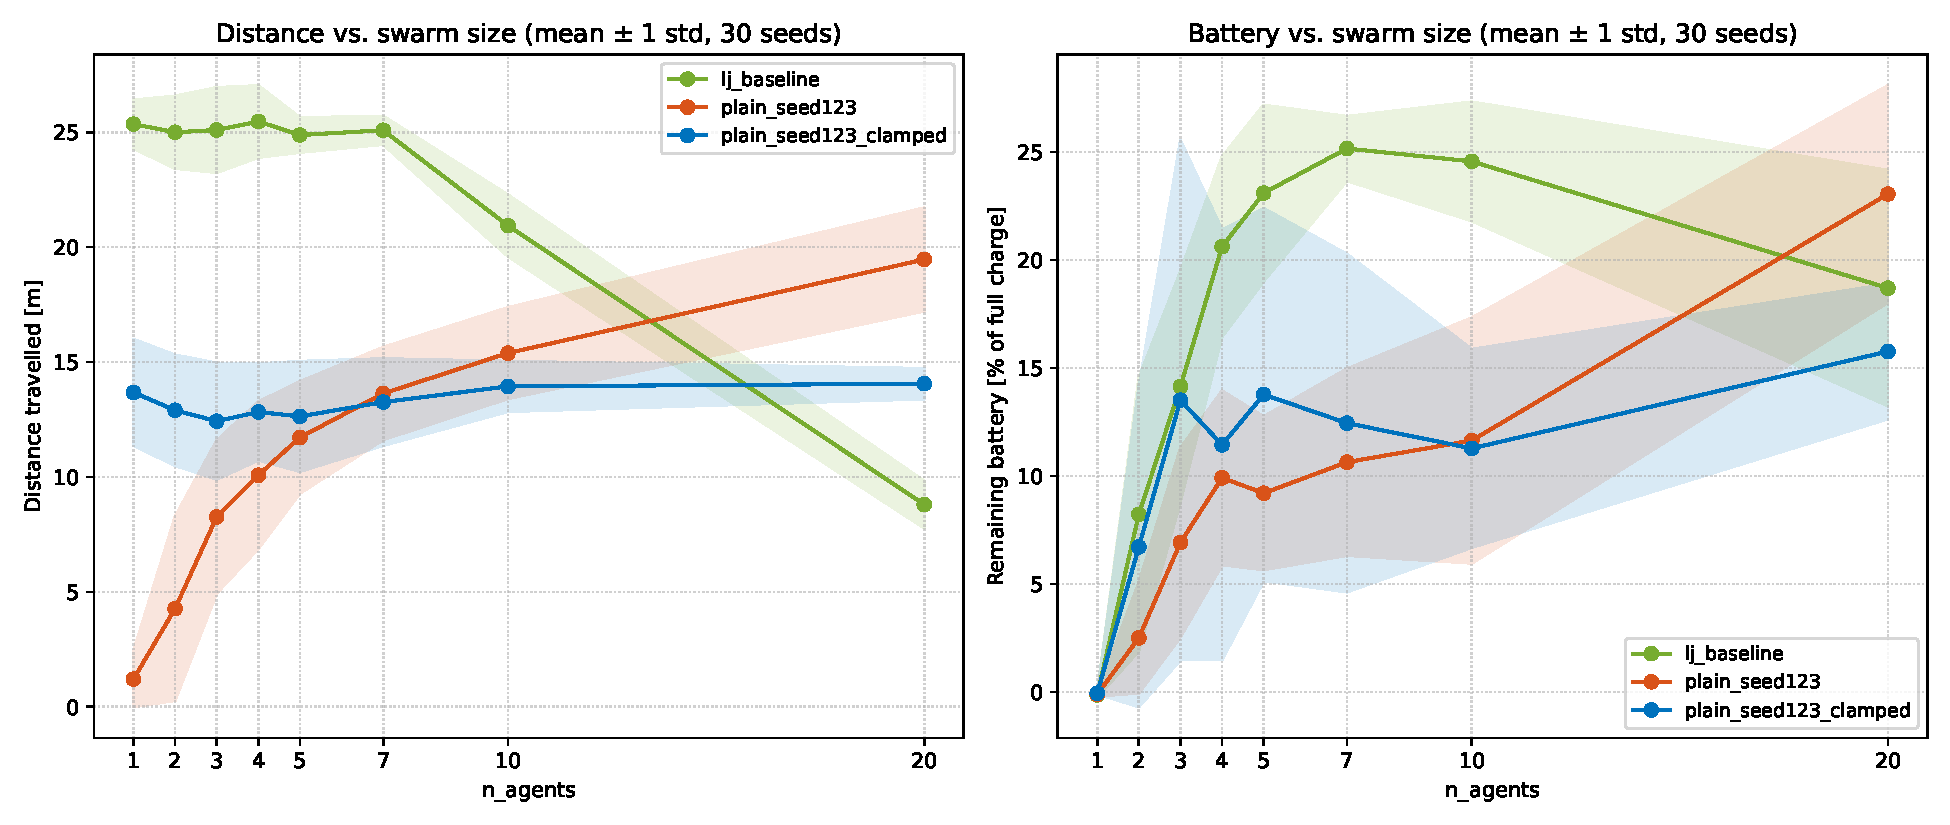
\includegraphics[width=\linewidth]{figures/n_agents_sweep_distance_battery_plain_seed123}
  \caption{\rev{Distance (left) and remaining battery (right) against swarm size, mean $\pm$ one standard deviation over 30 simulations per size, for the baseline (green) and the stage-2 controller evolved without (orange) and with (blue) the safety mechanisms. Both controllers were evolved with 20 robots.}}
  \label{fig:swarm_size}
\end{figure}


\begin{figure}[t]
  \centering
  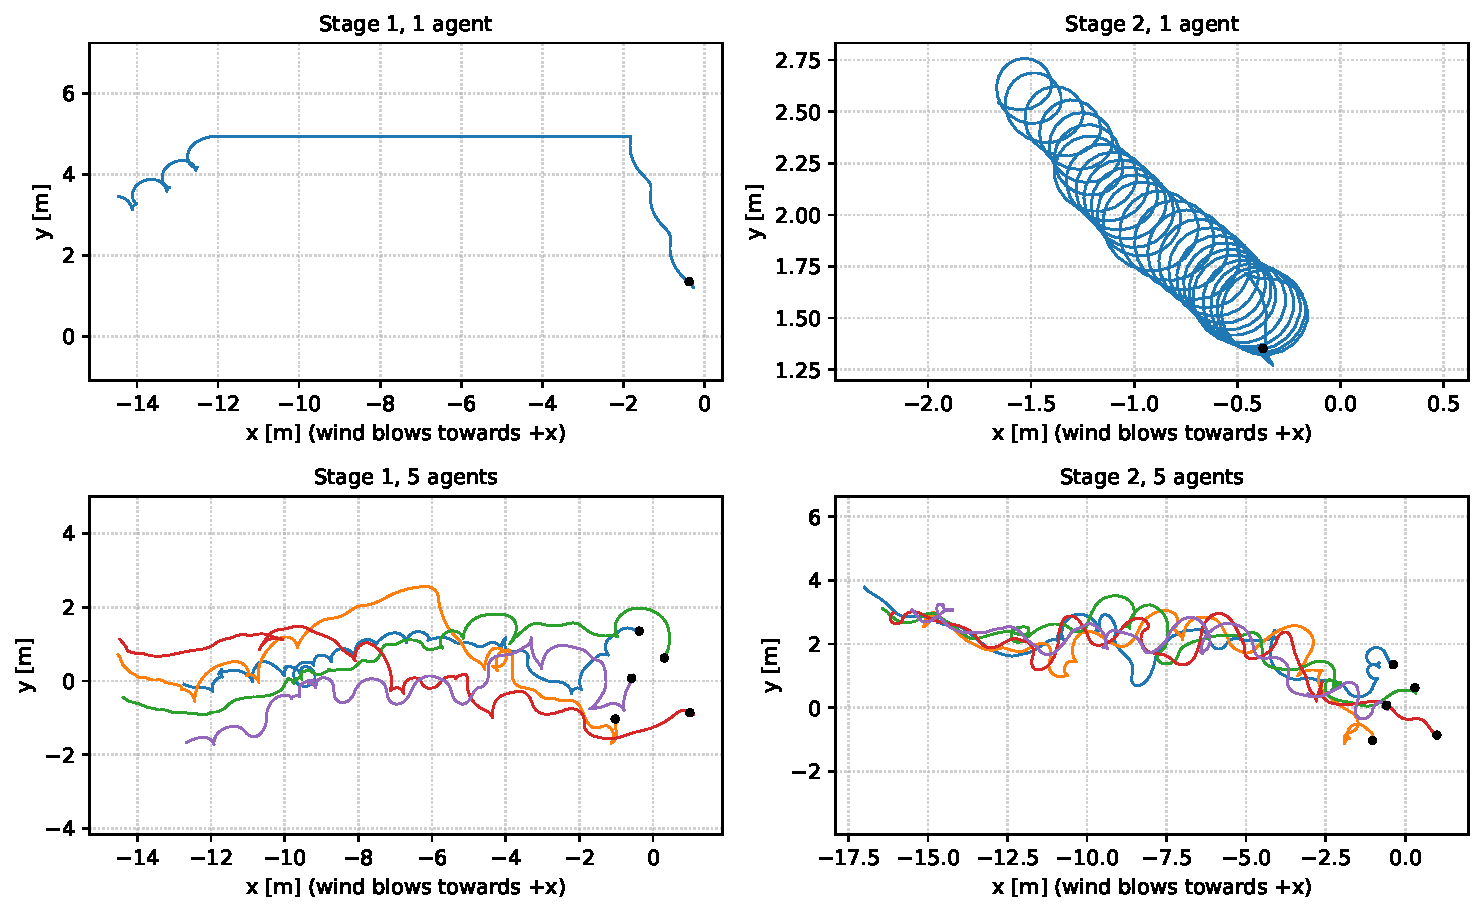
\includegraphics[width=\linewidth]{figures/paper_trajectories_stage1_vs_stage2}
  \caption{\rev{Trajectories of the best controller from stage 1 (left) and stage 2 (right) with one (top) and five (bottom) agents; black dots mark the starting positions. Note the different axis scales in the top-right panel.}}
  \label{fig:Debunk_Compass}
\end{figure}

The source code and the supplementary video are available in the Zenodo repository at \url{https://doi.org/10.5281/zenodo.18602800}.
\todo[inline]{Update the Zenodo release (code, controllers, supplementary video) to the two-stage version and replace this link.}



\section{Conclusion}
\label{sec:Conclusion}

We studied energy-efficient collective motion in a swarm of simple, memory-less ground robots. The swarm demonstrated emergent formation and dynamic formation reconfiguration, without these behaviours being explicitly encoded in the fitness function. Using a neural network controller with standard Hebbian plasticity, whose parameters were evolved via CMA-ES, the swarm learned to exploit local sensory readings and internal battery monitoring without explicit communication or wind sensing. \rev{With 20 robots, the resulting controller travelled $127\%$ further on average than a flocking baseline while also keeping more battery, and a version evolved with a speed clamp for safe use on real robots still travelled $59\%$ further. This advantage only appears in large swarms: with 12 or fewer robots the baseline performs better, and a single robot with the evolved controller hardly moves.} \rev{In the evolved swarm the front position changes hands about ten times per minute, almost five times as often as in the baseline, although robots do not cycle evenly between front and back.} A dedicated battery-awareness test showed that low-charge robots adapt by taking a conservative strategy through shielding themselves with other robots. Future works will investigate the minimal sensing and controller requirements that can manifest similar results\rev{, and how to evolve controllers that work across swarm sizes, for example by evaluating each candidate on several swarm sizes during evolution}. In addition, the impact of battery awareness on the learned strategies needs to be further investigated. For this matter, it is necessary to evolve a swarm that does not incorporate battery monitoring and see if similar behaviours can emerge.



%It was successfully shown that in a swarm of memory-less ground-robots, energy-efficient flocking and leader switching emerges through local interactions by making the agents battery-aware. We showed that that our NN controller whose weights are updated through Hebbian learning managed to realize these goals provided the right sensory inputs. Our work provides one possible solution to achieving the mentioned energy-efficient behaviours. A reasonable direction to go from here would be to do an ablation study to find out the minimum set of inputs necessary to achieve the same patterns.

\begin{credits}

\subsubsection{\ackname}
This work is supported in part by the NYUAD Center for Artificial Intelligence and Robotics (CAIR), funded by Tamkeen under the NYUAD Research Institute Award CG010, and by the NYUAD Center for Interdisciplinary Data Science \& AI (CIDSAI), funded by Tamkeen under the NYUAD Research Institute Award CG016.

\subsubsection{\discintname}
The authors declare they have no competing interests.

\end{credits}




\bibliographystyle{splncs04}
\bibliography{mybibliography2}

\end{document}
